%  !TeX spellcheck = en_GB
%  WangSheying于2015/11/2整理,TJU北洋园校区
%  TeXLive2015+TeXstudio个人推荐,可在线升级usepackage,比较方便
%*****************************************************************************************
%  从这里开始到\begin{document}是导言区,称之为preamble
\documentclass[UTF8]{beamer}
\usepackage[UTF8]{ctex}                 %使用中文要添加,可解决中文文档输入
\usepackage{newtxtext,newtxmath}  %字重齐全的高质量数学字体
\usepackage{mathrsfs}             %大写ABC的花体使用命令是\mathscr{}
\usepackage{graphicx}             %添加图片
\usepackage{bm}                   %专门处理数学粗体的bm宏包,使用命令是\bm{}
\usepackage{extarrows}            %延长符号,可在=,->等符号加多个字母
%\usepackage{amstext}              %它定义命令 \text,可用于在数学公式中插入少量文本,并可调整上下标中文本字体的尺寸。
\usepackage{amsthm}               %它定义了一个 proof 环境,用来排版定理和证明,能自动在最后添加证毕符号。它还提供一个命令:\newtheorem{定理环境名}{标题}[计数器名],可自定义定理类 环境
\usefonttheme{professionalfonts}  %这个更好看些,数学字体
\usepackage{indentfirst}          %首行缩进
\usepackage{amsmath}
\usepackage{amsfonts}
\usepackage{amssymb}
\usepackage{xcolor}
\usepackage{subfigure}
\usepackage[english]{babel}
\usepackage{algorithm}
\usepackage{algorithmic}
\usepackage{tikz}
\setlength{\parindent}{2em}      %首行缩进2字符
\setbeamertemplate{theorems}[numbered]
\setbeamertemplate{caption}[numbered]
%******************************************************************************************
%            以上是各种宏包
%******************************************************************************************
%下面是定理,定义,引言的声明,可自行添加

\newtheorem{thm}{Theorem}
%\newtheorem{lem}[thm]{Lemma}
\newtheorem{cor}[thm]{Corollary}
\newtheorem{prop}[thm]{Proposition}
\newtheorem{defi}[thm]{Definition}
\newtheorem{remark}[thm]{Remark}
\newtheorem{claim}[thm]{Claim}

\newenvironment{proofnoqed}{\begin{proof}<span style="background-color: rgb(255, 0, 0);">\renewcommand{\qedsymbol}{}  }{\end{proof} }
%有的证明比较长,前面的应该没有证毕符号,只在最后一个用proof,其他应该用自定义的新环境proofnoqed



%  三种颜色   red  purple   magenta





%上面是定理,定义,引言的声明,可自行添加
%******************************************************************************************
%下面是beamer的主题设置,目录框架结构,其实就是标题,目录等在上下左右哪一个位置放置,以及目录怎么显示
\usetheme{Singapore}            % 幻灯片模板选择singapore
\usecolortheme{sidebartab}      % 幻灯片模板的色彩sidebartab

\AtBeginSection[]{              % 幻灯片框架% 在每个Section前都会加入的Frame,
	\begin{frame}[plain]
		\frametitle{Outline}
		\tableofcontents[sectionstyle=show/shaded,subsectionstyle=show/show/shaded]
	\end{frame} 
}
%  \tableofcontents[comma-separated option list]具体讲解见《The beamer class User Guide》,
%  http://texdoc.net/texmf-dist/doc/latex/beamer/doc/beameruserguide.pdf     See in section 10.5 Adding a table of contents.
%  section和subsection相互独立,显示效果互不相关,Allowed ⟨styles⟩ are show, shaded, and hide
%  sectionstyle=⟨style for current section⟩/⟨style for other sections⟩
%  subsectionstyle=⟨style for current subsection⟩/⟨style for other subsections in current section⟩/⟨style for subsections in other sections⟩
%
% 上面是beamer的主题设置,目录框架结构,其实就是标题,目录等在上下左右哪一个位置放置,以及目录怎么显示
%*******************************************************************************************
%       下面标题页的内容设置,根据实际情况修改即可
\title{Spark 技术分享}  % 幻灯片封面
\author{王社英}
\institute{
	金融科技部/纳米科技\\
	wangsheying@wecash.net
}

\date{\today}  

%\date{9月 23, 2019}%一般是\today
%      上面标题页的内容设置根据实际情况修改即可
%*******************************************************************************************
%  \begin{document}以上是导言区,称之为preamble
%*******************************************************************************************
\begin{document}
	\begin{frame}[plain]
		%plain格式使得一帧的最上面是白色的,没有plain,会有色彩
		\titlepage
	\end{frame}
	\begin{frame}[plain]               % 幻灯片目录
		\frametitle{Outline}
		\tableofcontents[sectionstyle=show/show,subsectionstyle=show/show/hide]
	\end{frame}
	%The beamer class这本小册子有目录格式的讲解,sectionstyle,subsectionstyle都有,P100页
	%User Guide for version 3.36. 文档可在google搜索The beamer class,即可得到
%  以上是标准的配置,还有最下面的一部分标准配置
%********************************************************************************************
%    一帧的具体格式样例参考
%\section{节的名字}
%\subsection{小节的名字}
%\begin{frame}[plain,t]{节的名字} %也可以使用\frametitle{节的名字}效果一样
%	\structure{小节的名字} \\  \vspace{2ex}
%	节的名字正上方居中,小节的名字紧下方居左。
%\end{frame}
%*********************************************************************************************
%                  下面就是正文,自己的内容
%*********************************************************************************************

\section{Spark Introduction}
\subsection{A unified analytics engine}
\begin{frame}[plain,t]{Spark Introduction} %也可以使用\frametitle{节的名字}效果一样
	\structure{Spark Introduction} \\  \vspace{2ex}
     Apache Spark is a unified analytics engine for large-scale data processing.
     
     \vspace{2ex}
     
     You can run Spark using its standalone cluster mode, on EC2, on Hadoop YARN, on Mesos, or on Kubernetes. 
     
      \vspace{2ex}
      
     Access data in HDFS, Alluxio, Apache Cassandra, Apache HBase, Apache Hive, and hundreds of other data sources.
     
     
    
\end{frame}
\begin{frame}[plain,t]{Spark Introduction} %也可以使用\frametitle{节的名字}效果一样
	\structure{Spark Introduction} \\  \vspace{2ex}
	\begin{figure}
		\centering
		
\includegraphics[width=0.7\linewidth]{images/intr002}
		\label{fig:intr002}
	\end{figure}
	
\end{frame}
\begin{frame}[plain,t]{Spark Introduction} %也可以使用\frametitle{节的名字}效果一样
	\structure{Spark Introduction} \\  \vspace{2ex}
	
	\begin{figure}
		\centering
		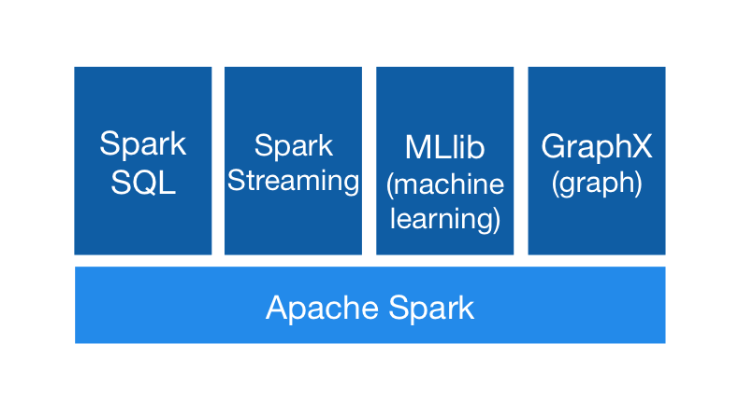
\includegraphics[width=0.7\linewidth]{images/intr001}
		\label{fig:intr001}
	\end{figure}
	
\end{frame}
\section{Spark Initialization}
\subsection{ApplicationMaster}
\begin{frame}[plain,t]{Spark Initialization} %也可以使用\frametitle{节的名字}效果一样
	\structure{Spark Submit} \\  \vspace{2ex}
	\begin{figure}
		\centering
		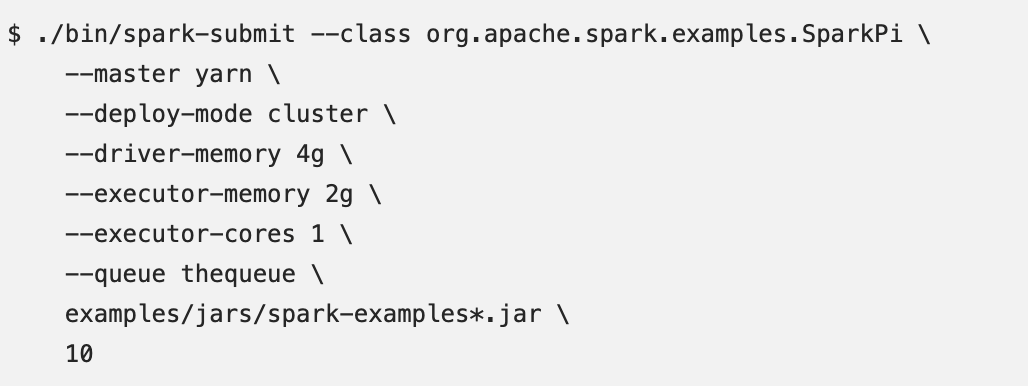
\includegraphics[width=0.9\linewidth]{images/app016}
		\label{fig:app016}
	\end{figure}
	\begin{figure}
		\centering
		
\includegraphics[width=0.9\linewidth]{images/app017}
		%\caption{}
		\label{fig:app017}
	\end{figure}
	
	
\end{frame}

\begin{frame}[plain,t]{ApplicationMaster} %也可以使用\frametitle{节的名字}效果一样
	\structure{ApplicationMaster Initialization} \\  \vspace{2ex}
	\begin{figure}
		\centering
		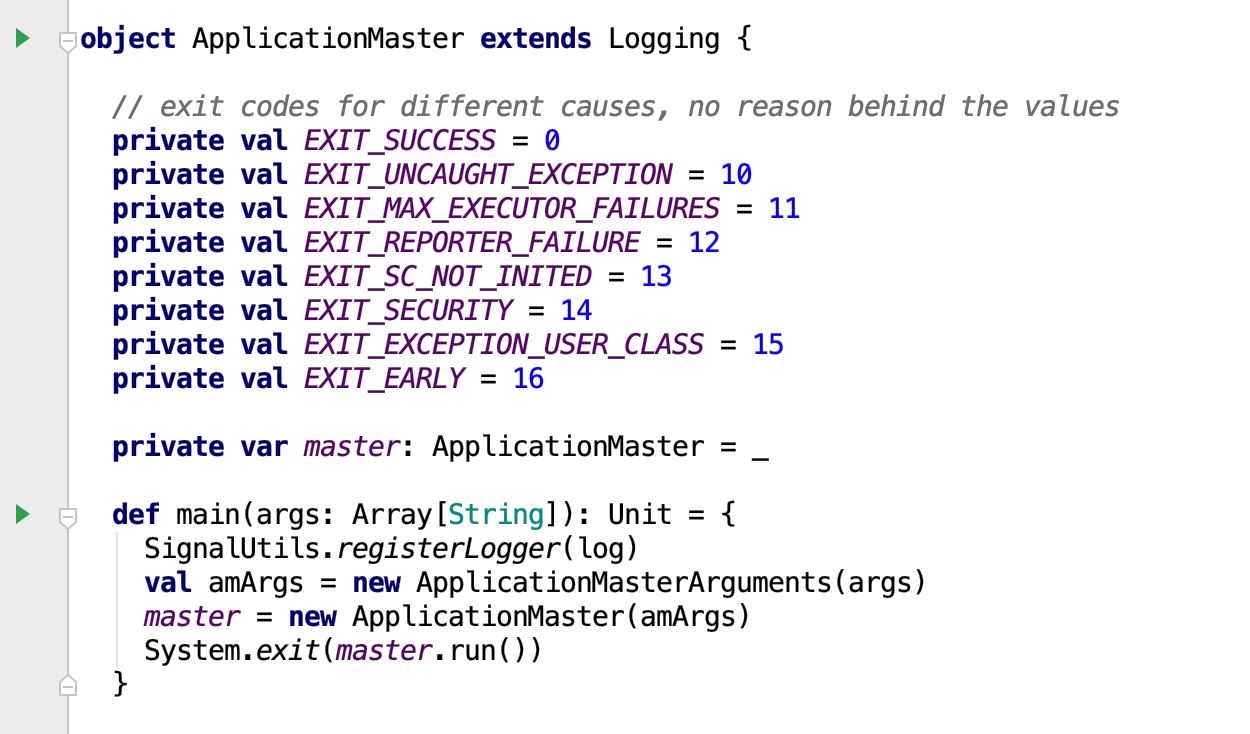
\includegraphics[width=0.9\linewidth]{images/app001}
		\caption{ApplicationMaster\#main}
		\label{fig:app001}
	\end{figure}
	

\end{frame}
\begin{frame}[plain,t]{ApplicationMaster} %也可以使用\frametitle{节的名字}效果一样
	\structure{ApplicationMaster Initialization} \\  \vspace{2ex}
	\begin{figure}
		\centering
		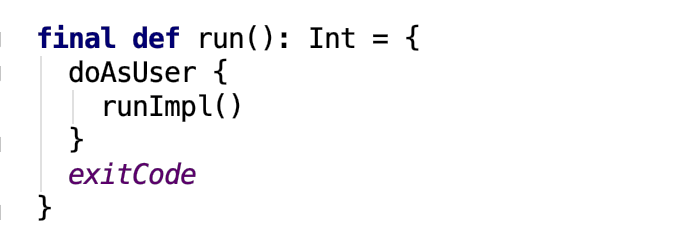
\includegraphics[width=0.9\linewidth]{images/app002}
		\caption{ApplicationMaster\#run}
		\label{fig:app002}
	\end{figure}
\end{frame}
\begin{frame}[plain,t]{ApplicationMaster} %也可以使用\frametitle{节的名字}效果一样
	\structure{ApplicationMaster Initialization} \\  \vspace{2ex}
	\begin{figure}
		\centering
		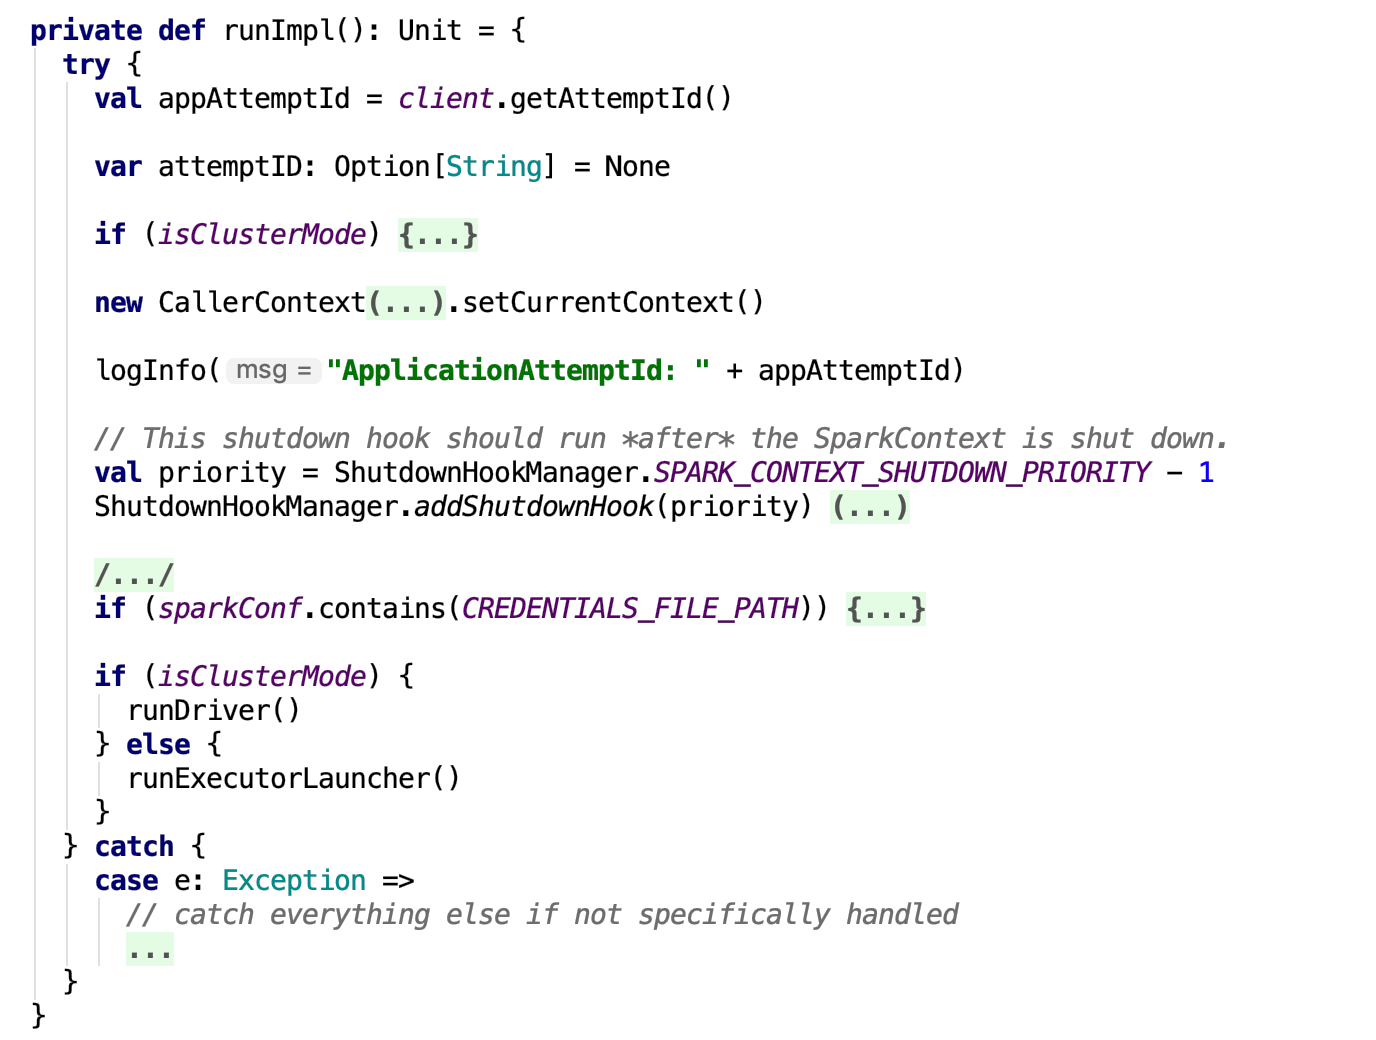
\includegraphics[width=0.8\linewidth]{images/app003}
		\caption{ApplicationMaster\#runImpl}
		\label{fig:app003}
	\end{figure}
	
	
\end{frame}
\begin{frame}[plain,t]{ApplicationMaster} %也可以使用\frametitle{节的名字}效果一样
	\structure{ApplicationMaster Initialization {\color{red} Cluster}} \\  
	\begin{figure}
		\centering
		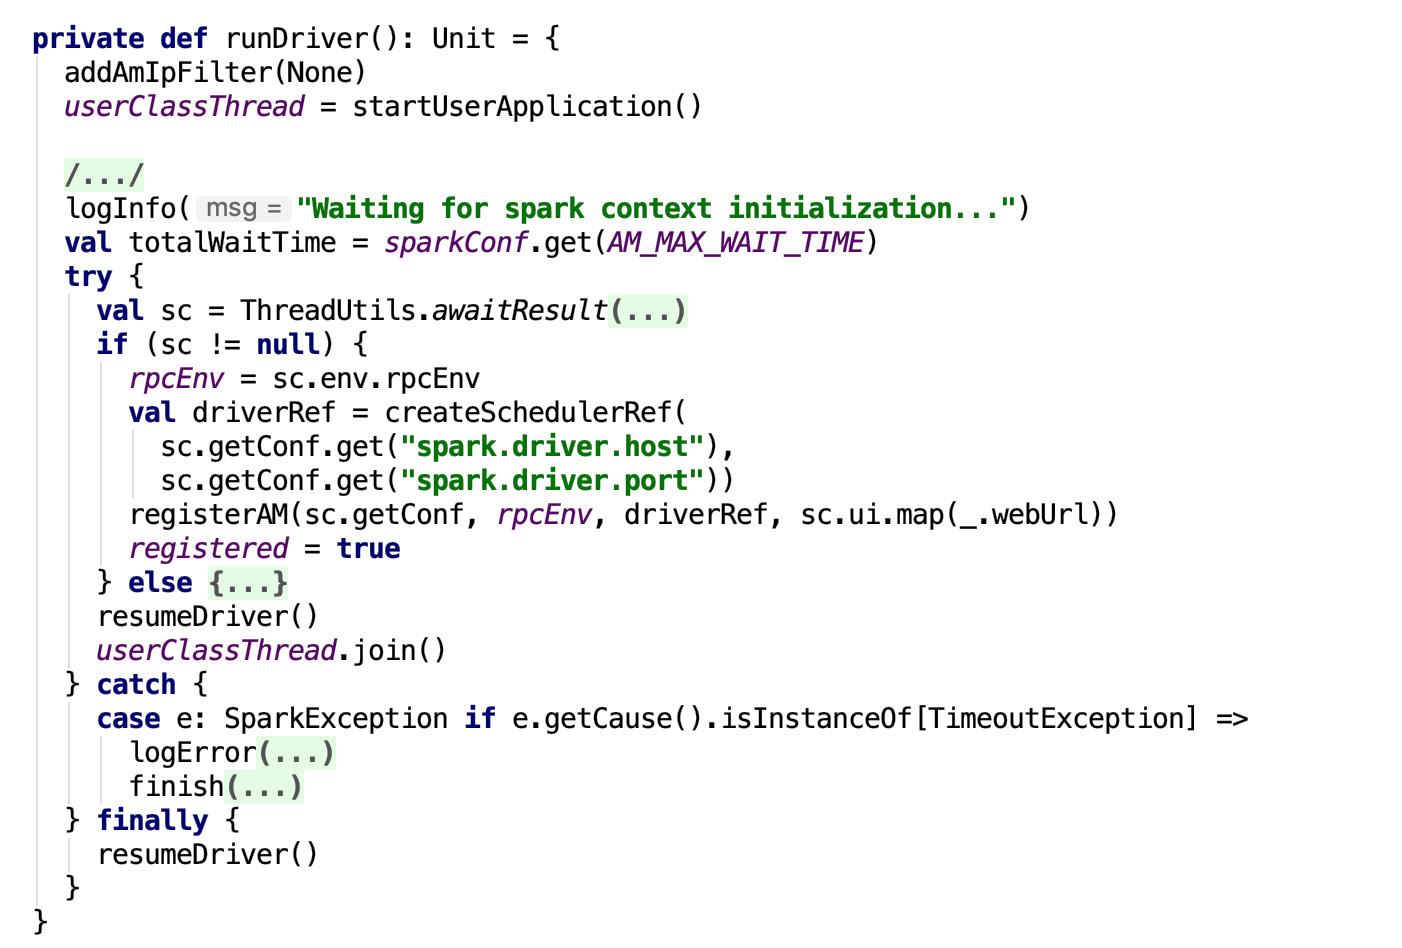
\includegraphics[width=0.9\linewidth]{images/app005}
		\caption{ApplicationMaster\#runDriver}
		\label{fig:app005}
	\end{figure}
	
\end{frame}
\begin{frame}[plain,t]{ApplicationMaster} %也可以使用\frametitle{节的名字}效果一样
	\structure{ApplicationMaster Initialization {\color{red} Cluster}} \\  
	\begin{figure}
		\centering
		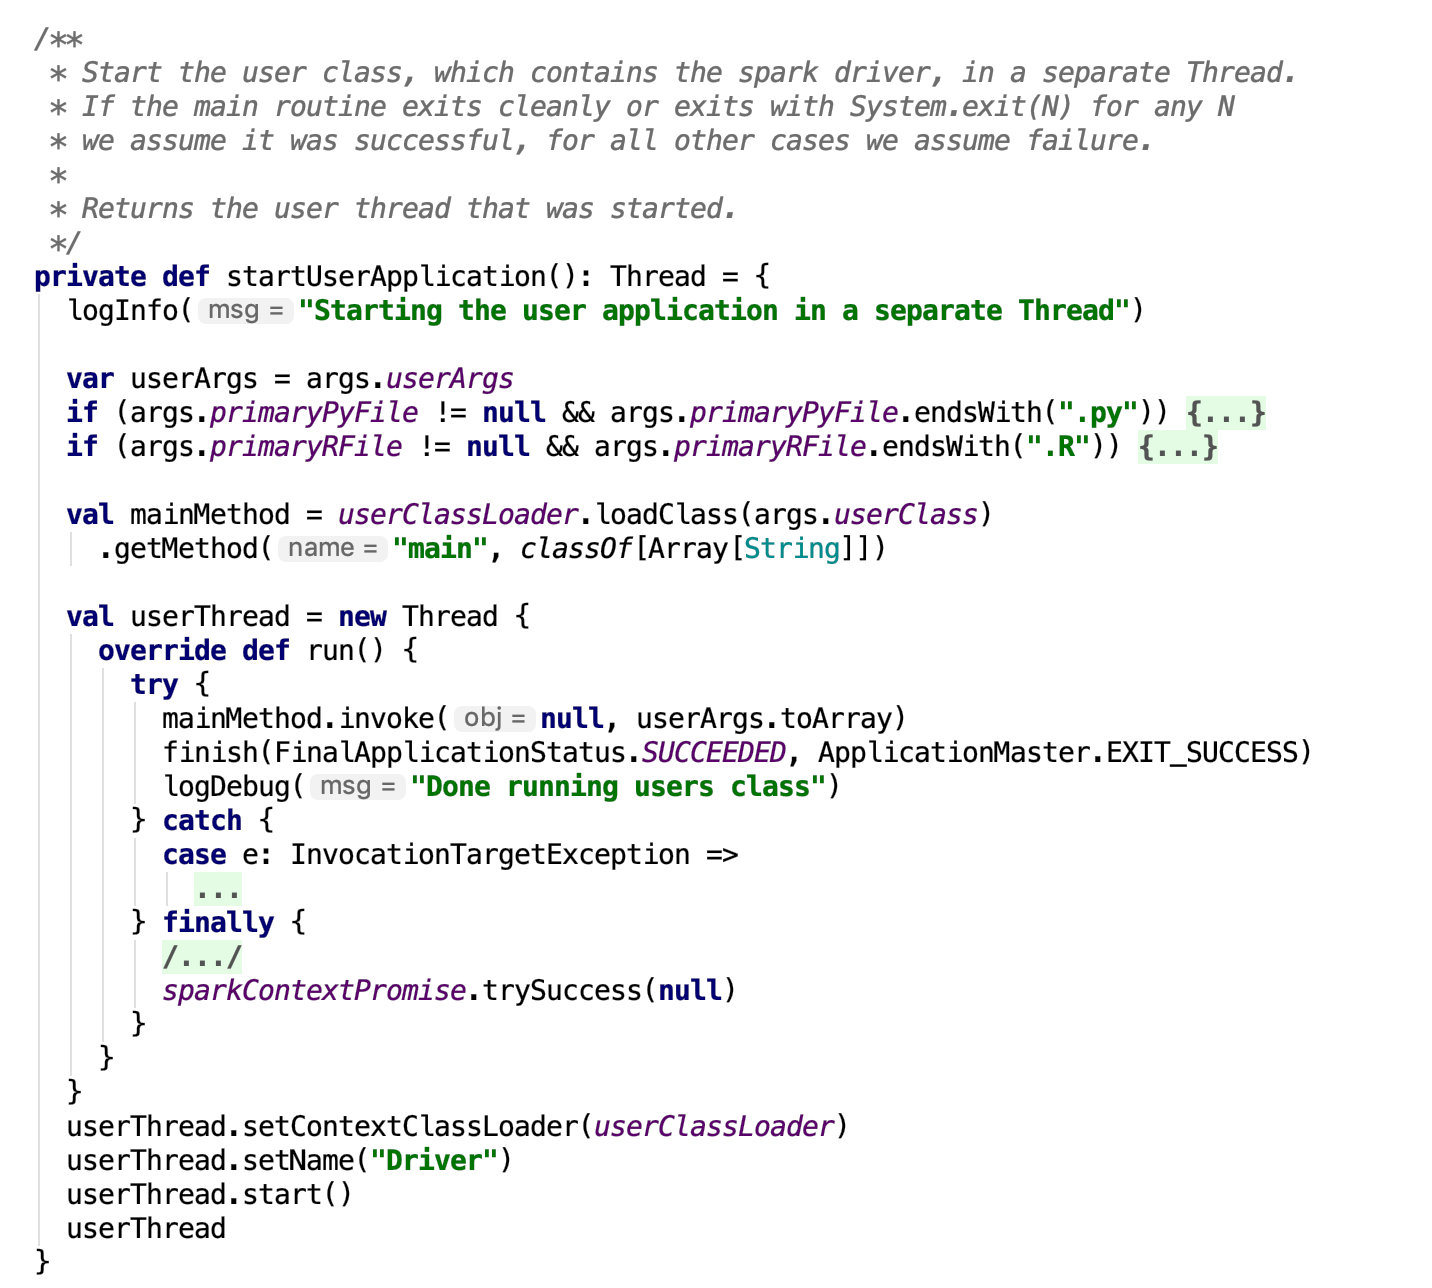
\includegraphics[width=0.8\linewidth]{images/app004}
		\caption{ApplicationMaster\#startUserApplication}
		\label{fig:app004}
	\end{figure}
	
\end{frame}
\begin{frame}[plain,t]{ApplicationMaster} %也可以使用\frametitle{节的名字}效果一样
	\structure{ApplicationMaster Initialization {\color{magenta} Client}} \\  \vspace{2ex}
	\begin{figure}
		\centering
		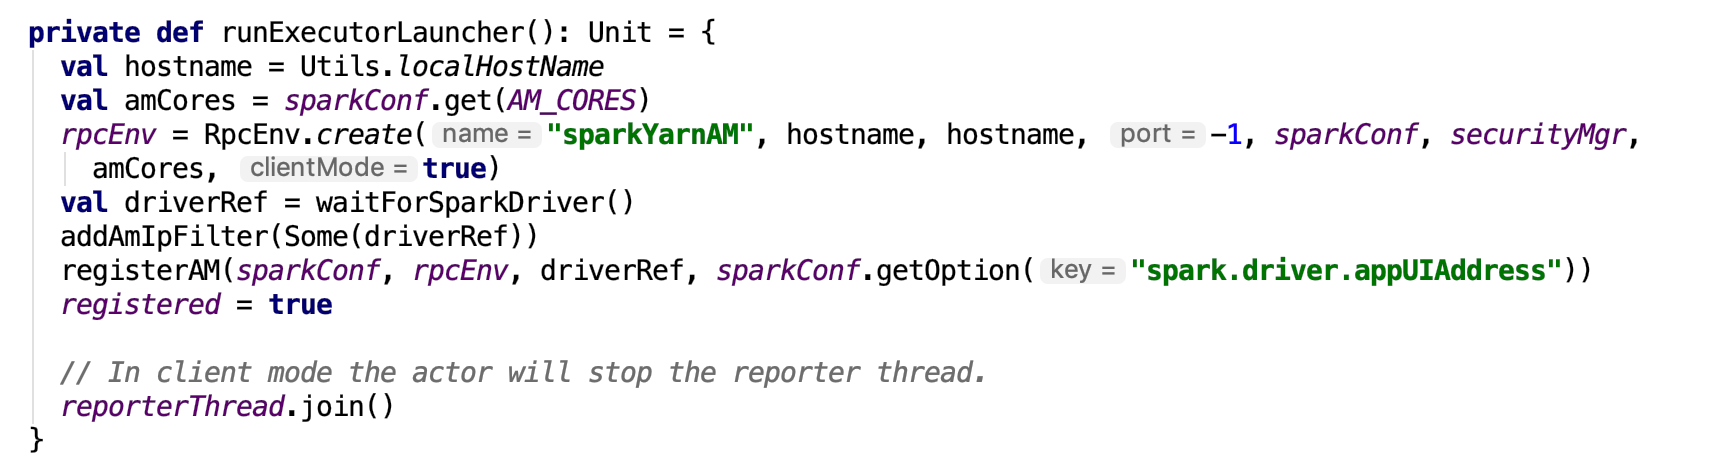
\includegraphics[width=0.9\linewidth]{images/app006}
		\caption{ApplicationMaster\#runExecutorLauncher}
		\label{fig:app006}
	\end{figure}
	
\end{frame}
\begin{frame}[plain,t]{ApplicationMaster} %也可以使用\frametitle{节的名字}效果一样
	\structure{ApplicationMaster Initialization {\color{magenta} Client}} \\  
	\begin{figure}
		\centering
		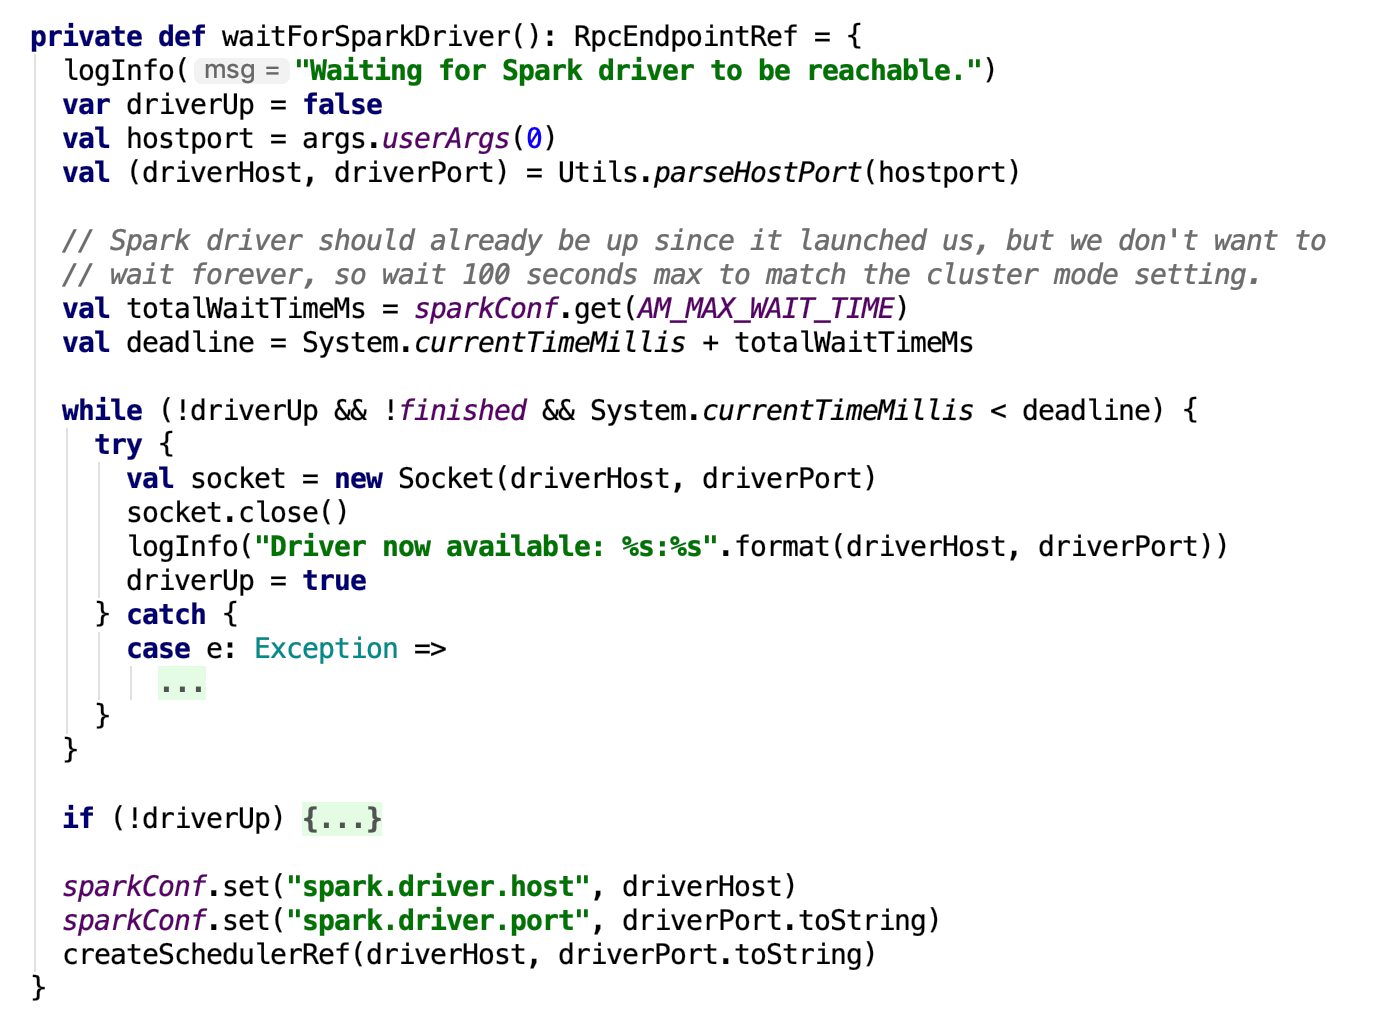
\includegraphics[width=0.85\linewidth]{images/app007}
		\caption{ApplicationMaster\#waitForSparkDriver}
		\label{fig:app007}
	\end{figure}
	
\end{frame}
\begin{frame}[plain,t]{ApplicationMaster} %也可以使用\frametitle{节的名字}效果一样
	\structure{Request Resources} \\ 
	\begin{figure}
		\centering
		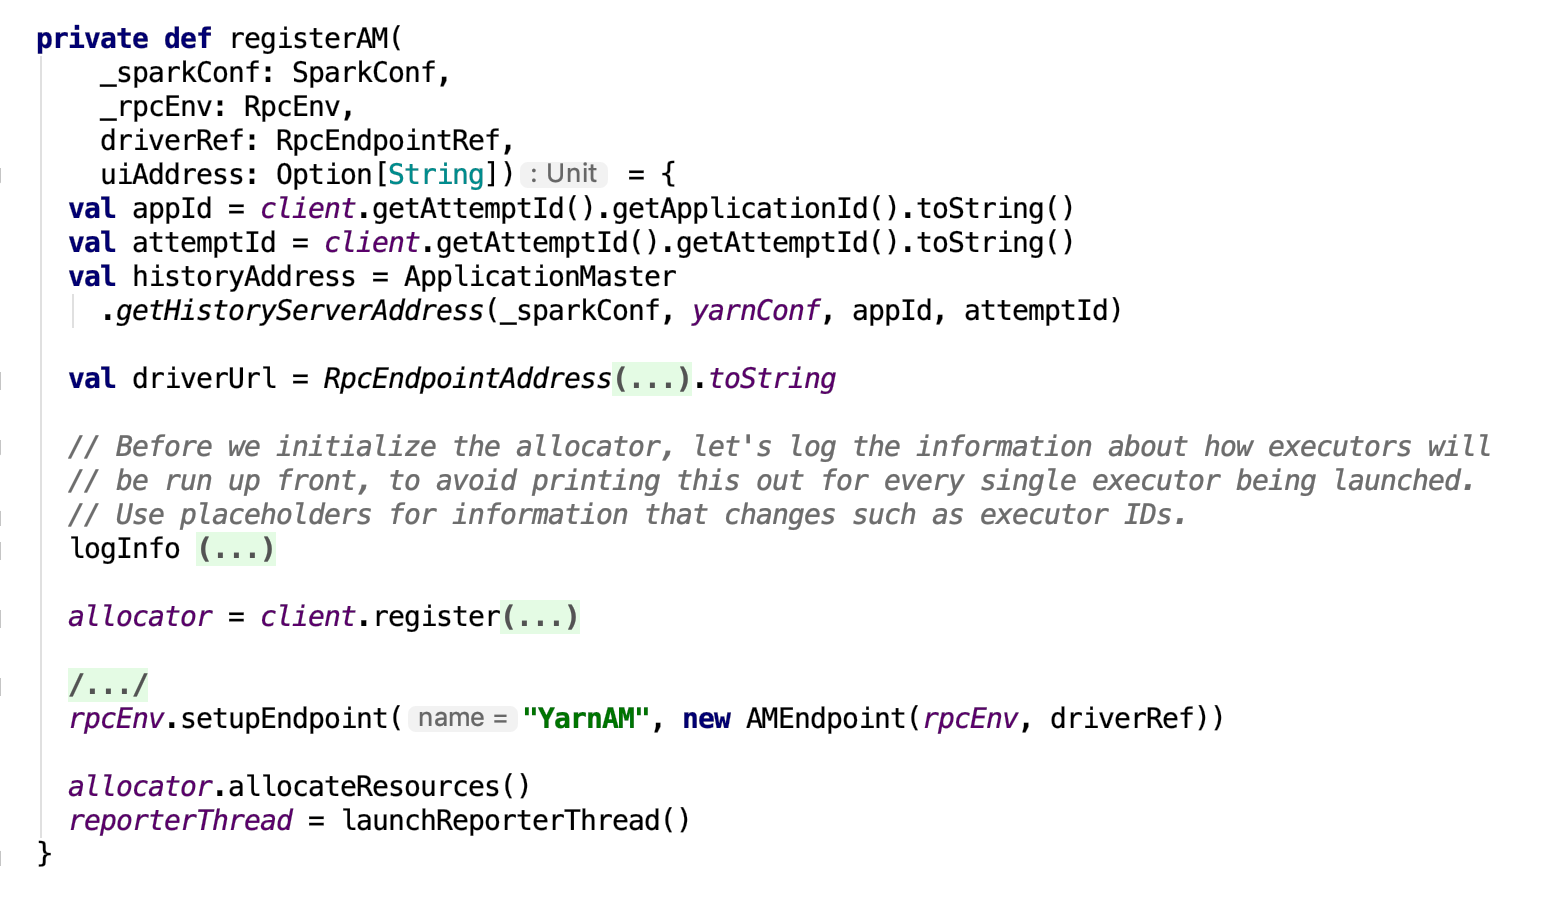
\includegraphics[width=0.9\linewidth]{images/app008}
		\caption{ApplicationMaster\#registerAM}
		\label{fig:app008}
	\end{figure}
	
\end{frame}
\begin{frame}[plain,t]{ApplicationMaster} %也可以使用\frametitle{节的名字}效果一样
	\structure{Request Resources} \\ 
	\begin{figure}
		\centering
		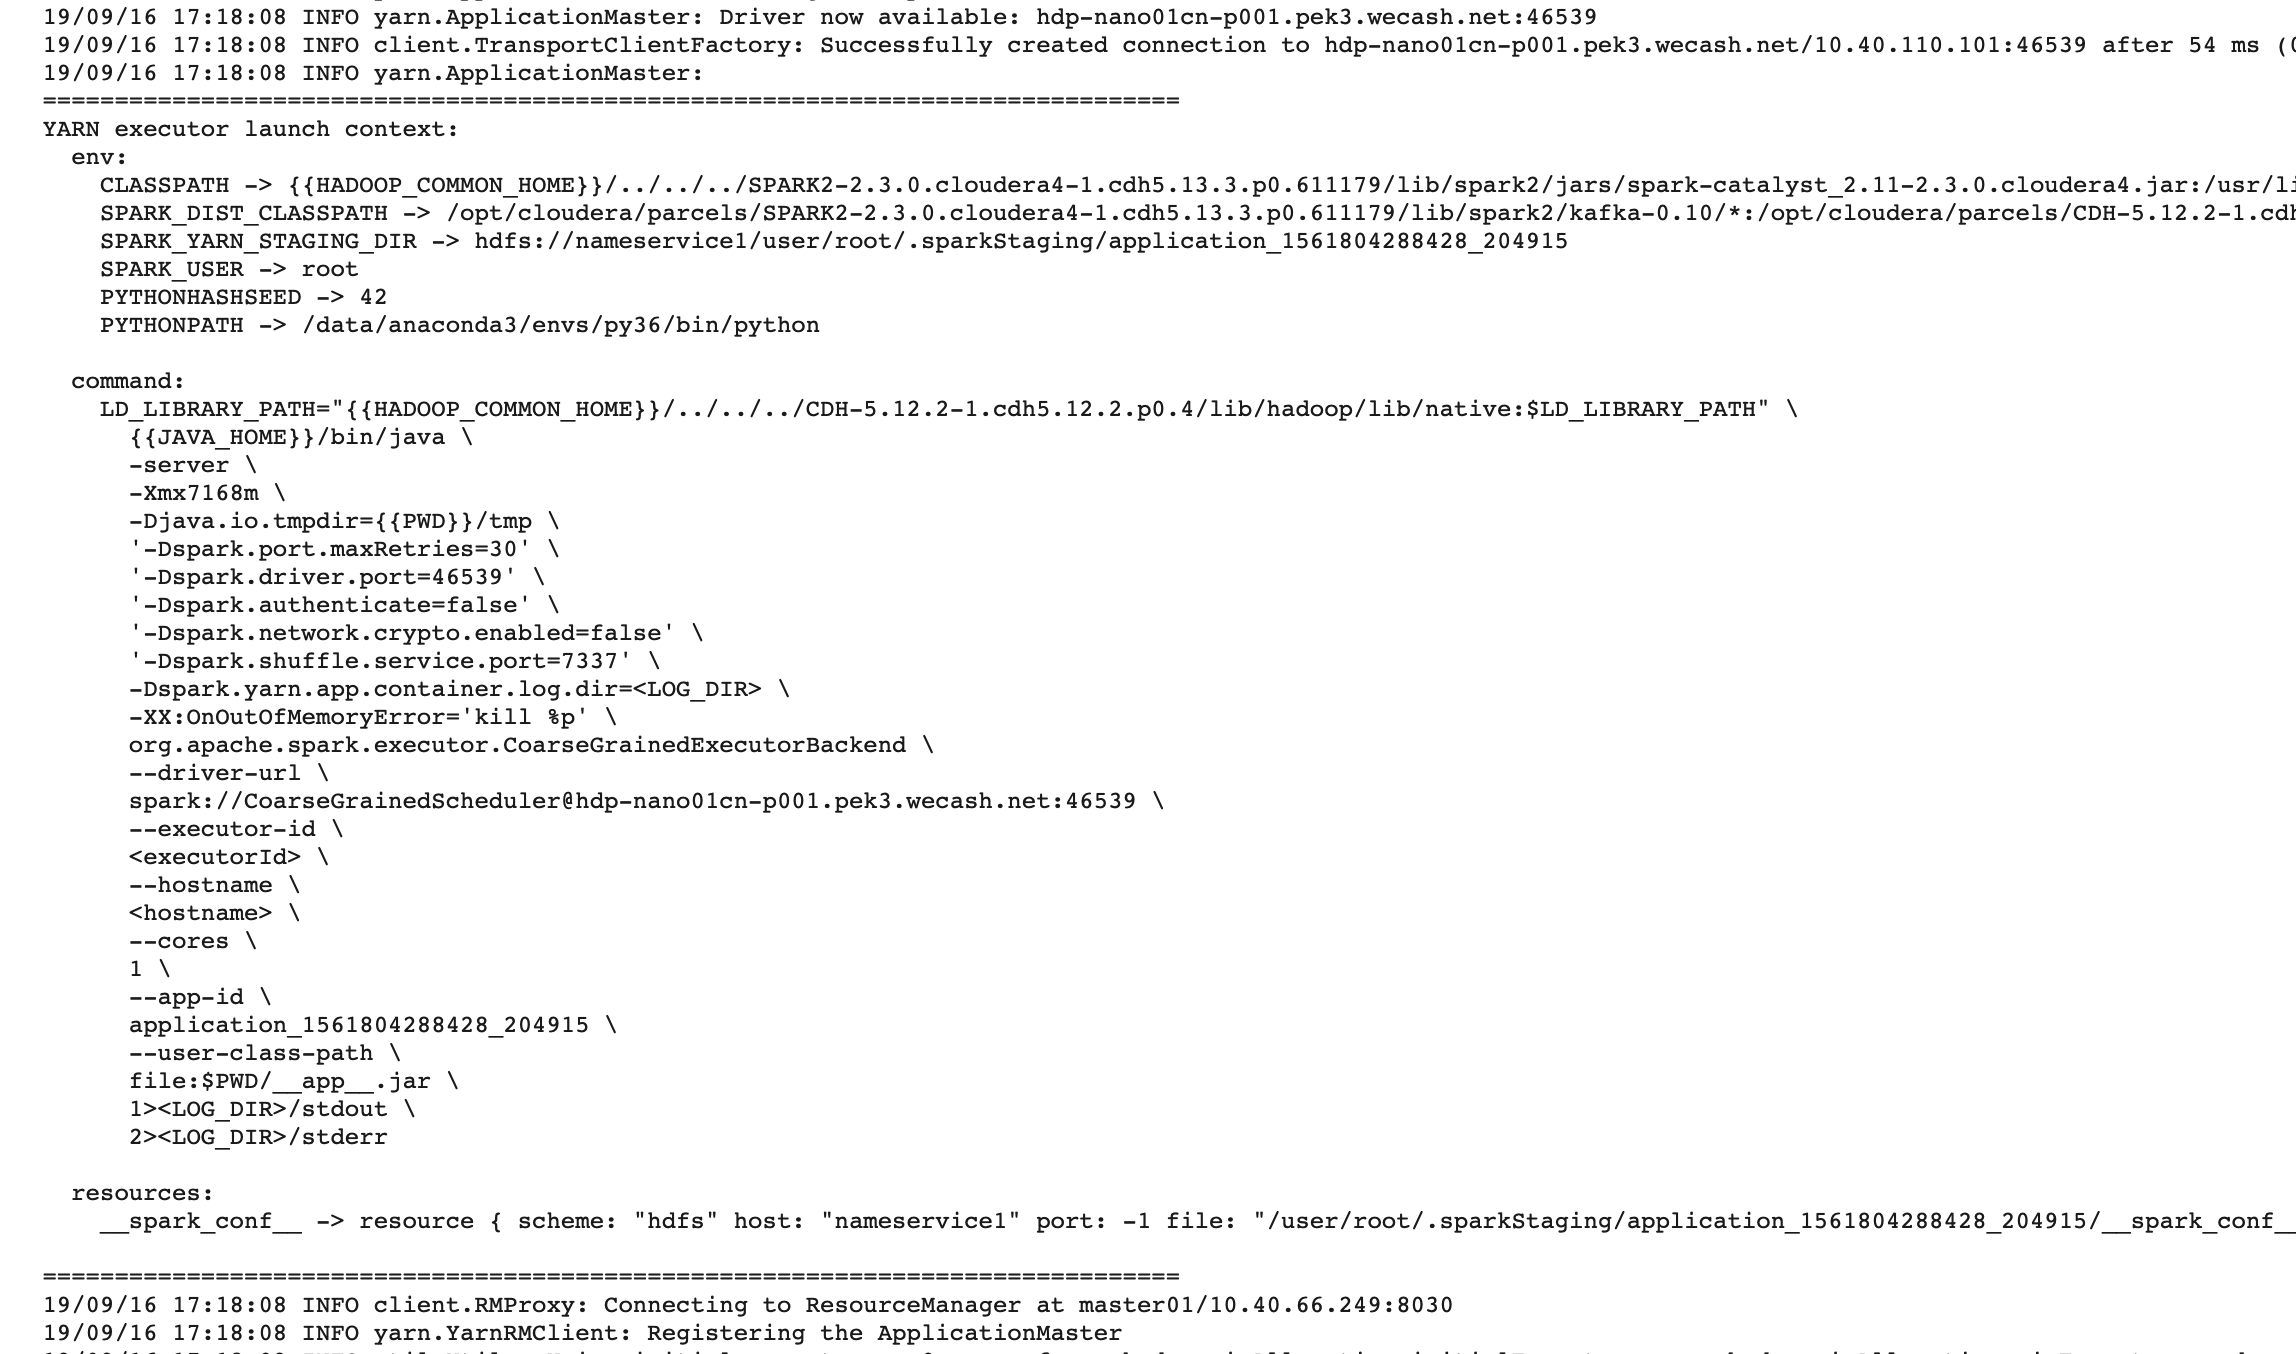
\includegraphics[width=0.9\linewidth]{images/app009}
		\caption{YARN executor launch context}
		\label{fig:app009}
	\end{figure}
	
	
\end{frame}
\begin{frame}[plain,t]{ApplicationMaster} %也可以使用\frametitle{节的名字}效果一样
	\structure{Request Resources} \\  \vspace{2ex}
	\begin{figure}
		\centering
		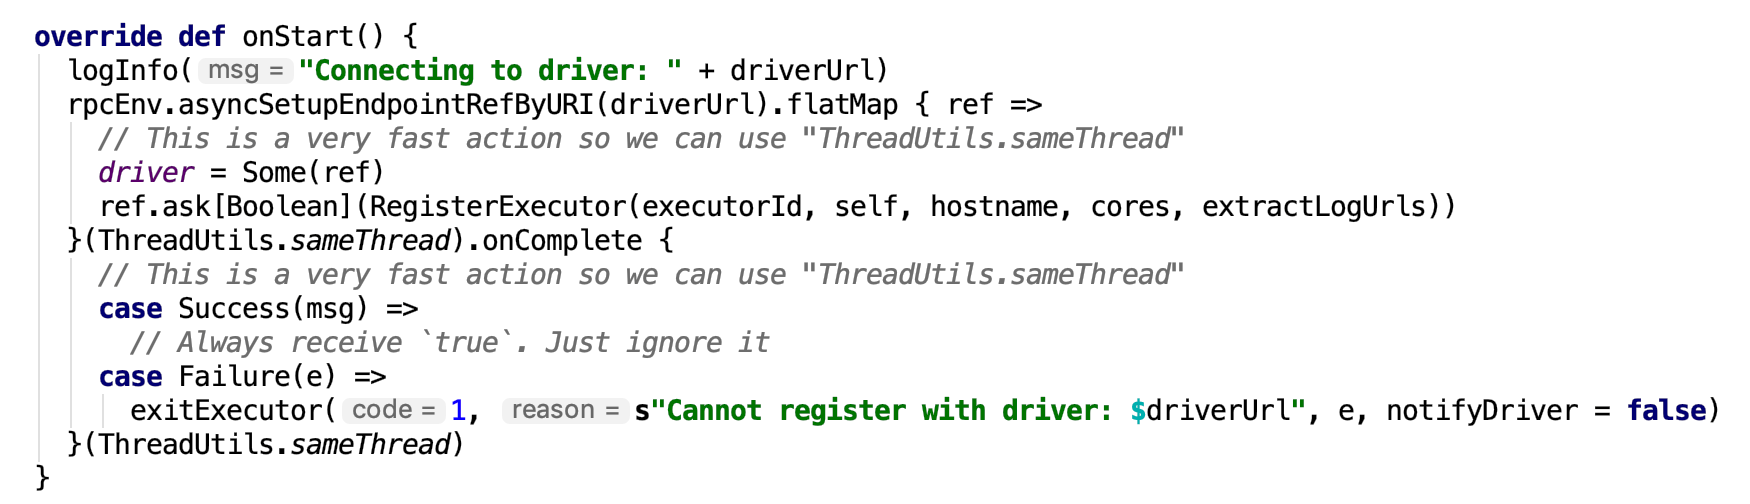
\includegraphics[width=0.9\linewidth]{images/app010}
		\caption{CoarseGrainedExecutorBackend\#onStart}
		\label{fig:app010}
	\end{figure}
	
	
\end{frame}
\begin{frame}[plain,t]{ApplicationMaster} %也可以使用\frametitle{节的名字}效果一样
	\structure{Request Resources} \\  \vspace{2ex}
\begin{figure}
	\centering
	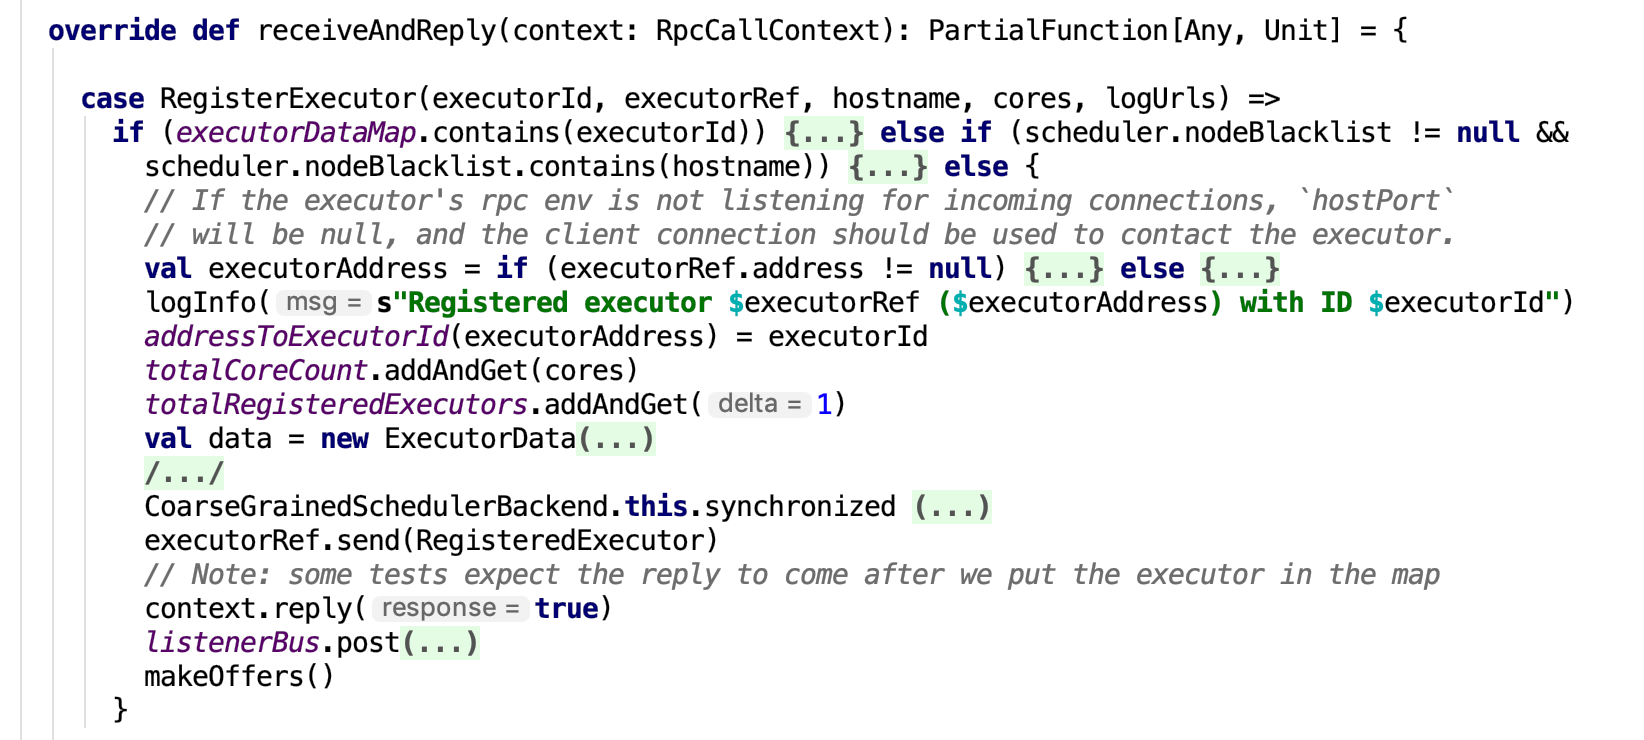
\includegraphics[width=0.9\linewidth]{images/app011}
	\caption{DriverEndpoint\#receiveAndReply}
	\label{fig:app011}
\end{figure}

\end{frame}
\begin{frame}[plain,t]{ApplicationMaster} %也可以使用\frametitle{节的名字}效果一样
	\structure{Request Resources} \\  
	\begin{figure}
		\centering
		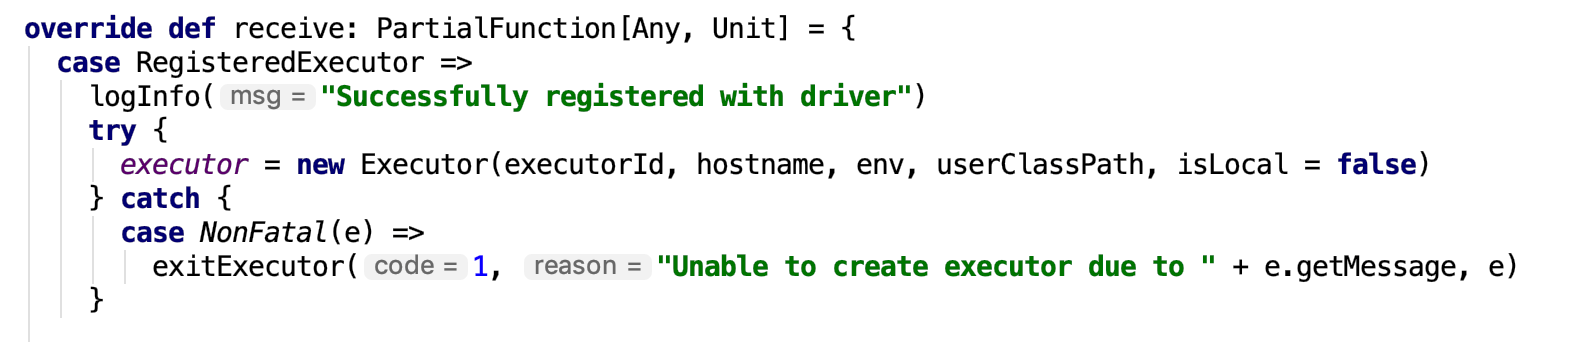
\includegraphics[width=0.9\linewidth]{images/app012}
		\caption{CoarseGrainedExecutorBackend\#receive}
		\label{fig:app012}
	\end{figure}
	\begin{figure}
		\centering
		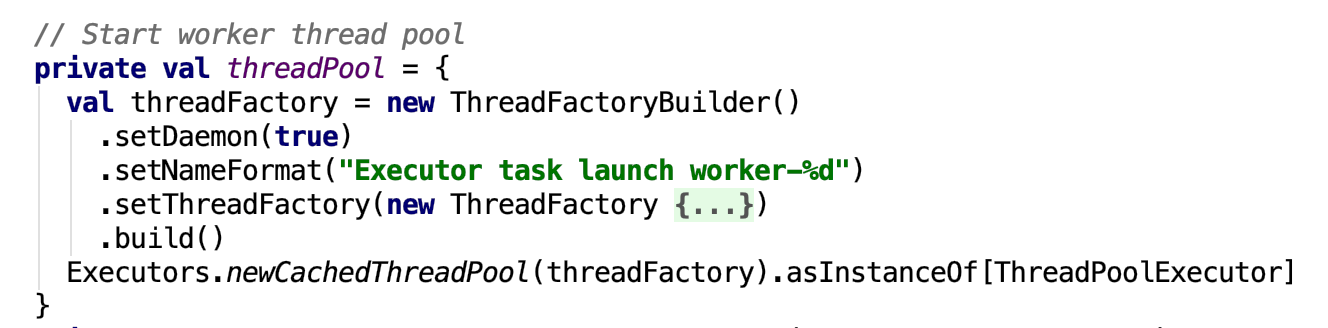
\includegraphics[width=0.9\linewidth]{images/app013}
		\caption{Executor\#threadPool}
		\label{fig:app013}
	\end{figure}
	
\end{frame}

\begin{frame}[plain,t]{ApplicationMaster} %也可以使用\frametitle{节的名字}效果一样
	\structure{Request Resources} \\  \vspace{2ex}
	\begin{figure}
		\centering
		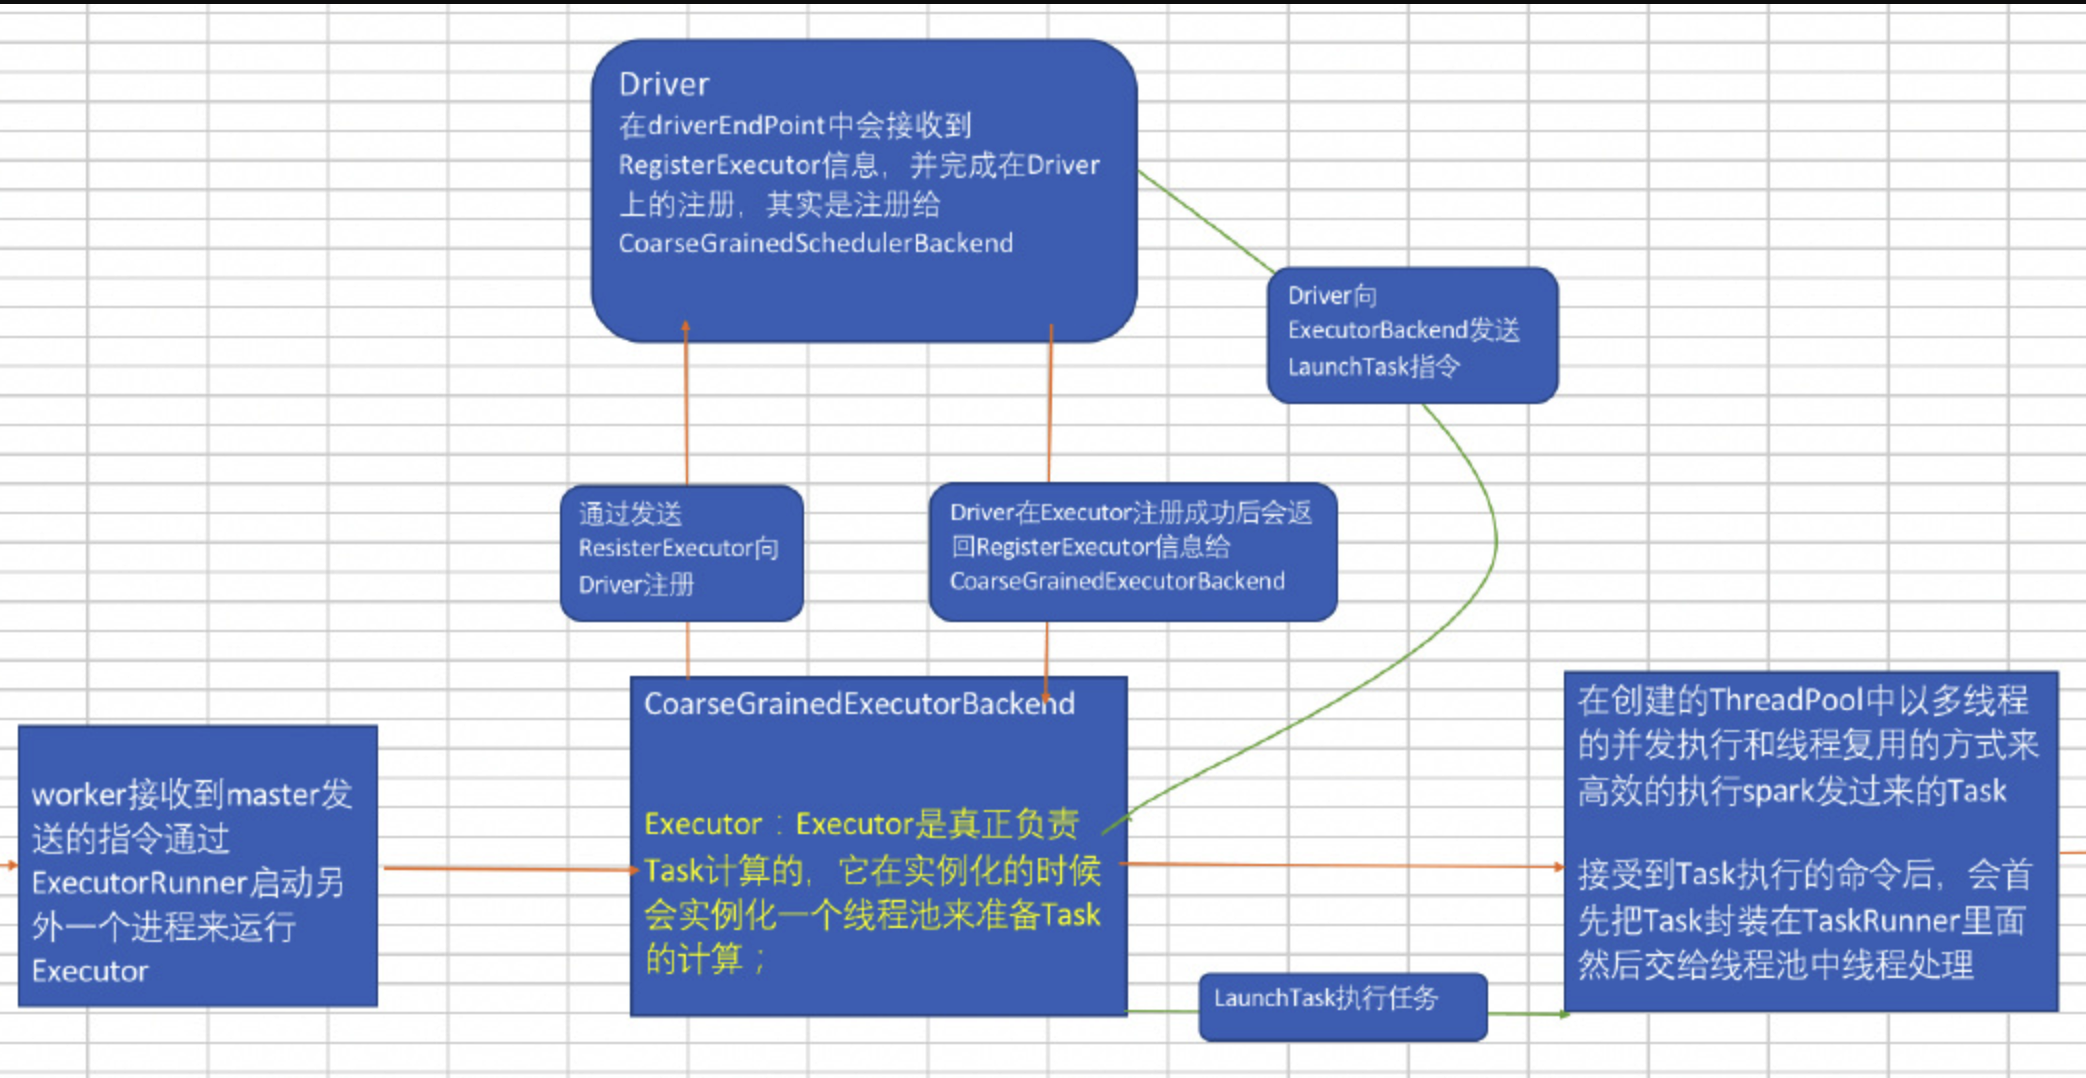
\includegraphics[width=0.9\linewidth]{images/init001}
		\caption{资源请求流程示意图}
		\label{fig:init001}
	\end{figure}
	
\end{frame}
\subsection{SparkContext}
\begin{frame}[plain,t]{SparkContext} %也可以使用\frametitle{节的名字}效果一样
	\structure{Main entry point for Spark functionality} \\  \vspace{2ex}
	A SparkContext represents the connection to a Spark
	 cluster, and can be used to create RDDs, accumulators and broadcast variables on that cluster.
	 
	 \vspace{2ex}
	 
	 \begin{itemize}
	 	\item LiveListenerBus
	 	\item TaskScheduler
	 	\item SchedulerBackend
	 	\item DAGScheduler
	 	\item MapOutputTrackerMaster
	 	\item BlockManagerMaster
	 \end{itemize}
\end{frame}
\begin{frame}[plain,t]{SparkContext} %也可以使用\frametitle{节的名字}效果一样
	\structure{SparkContext Initialization} \\  \vspace{2ex}
	\begin{figure}
		\centering
		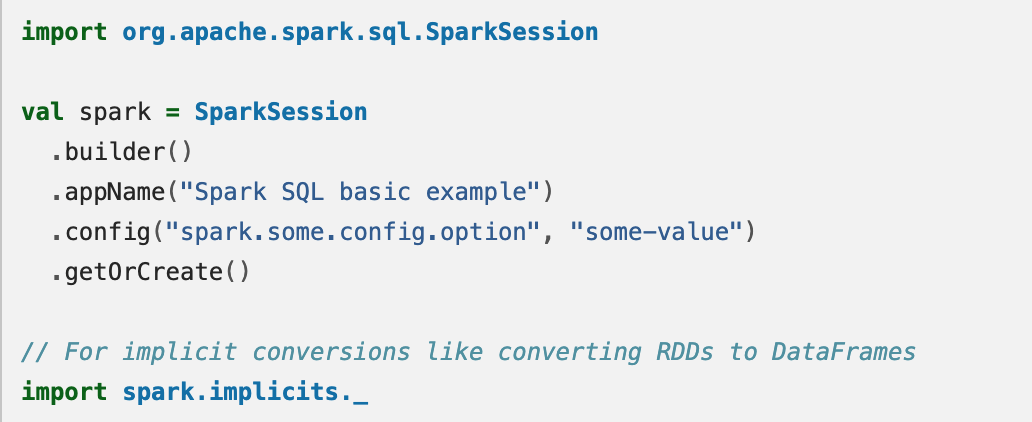
\includegraphics[width=0.9\linewidth]{images/app018}
		%\caption{}
		\label{fig:app018}
	\end{figure}
	
	
\end{frame}
\begin{frame}[plain,t]{SparkContext} %也可以使用\frametitle{节的名字}效果一样
	\structure{SparkContext Initialization} \\  \vspace{2ex}
	\begin{figure}
		\centering
		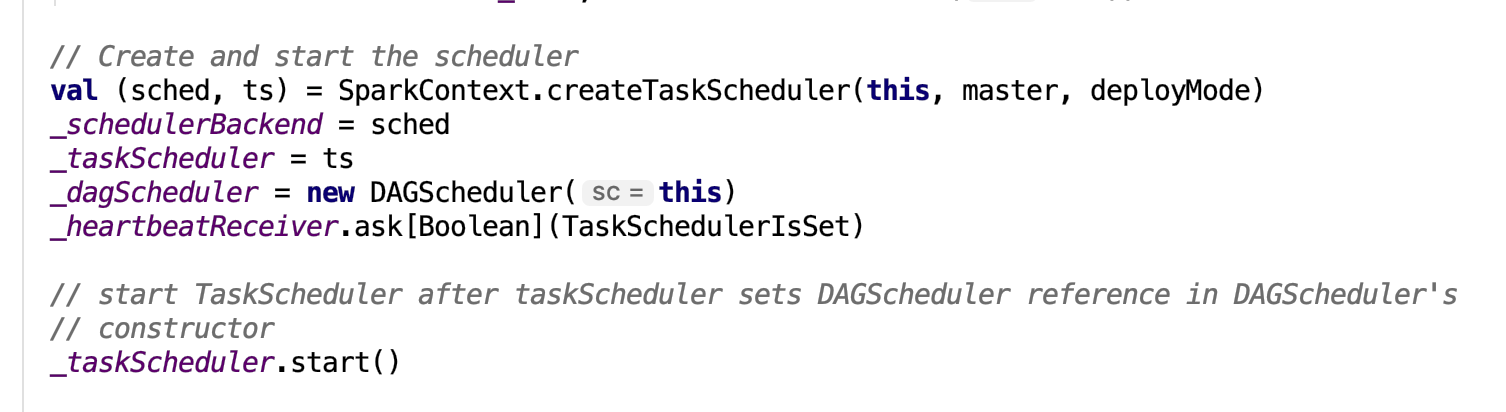
\includegraphics[width=0.9\linewidth]{images/init002}
		\caption{SparkContext\#init}
		\label{fig:init002}
	\end{figure}
	
\end{frame}


\begin{frame}[plain,t]{SparkContext} %也可以使用\frametitle{节的名字}效果一样
	\structure{Spark Local} \\ 
	\begin{figure}
		\centering
		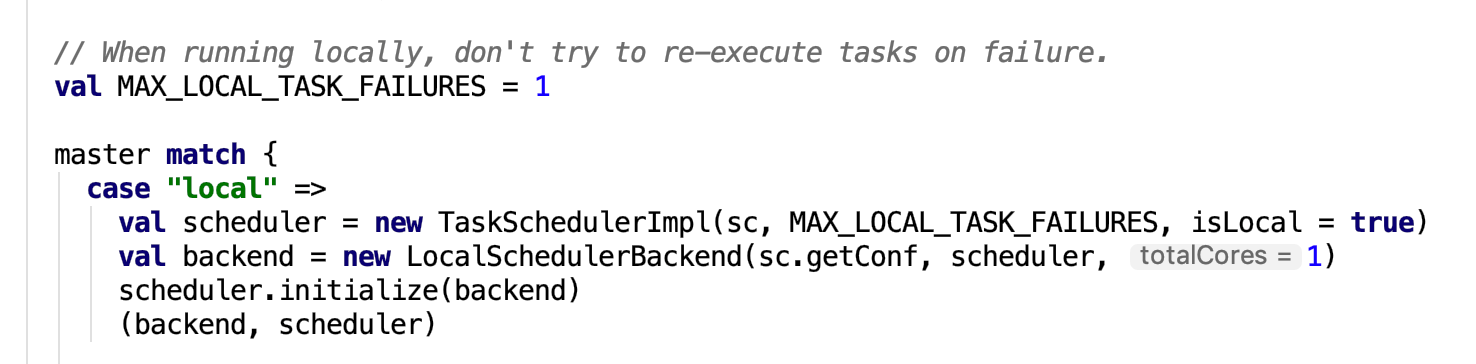
\includegraphics[width=0.9\linewidth]{images/init007}
		\caption{SparkContext\#createTaskScheduler}
		\label{fig:init007}
	\end{figure}
	\begin{figure}
		\centering
		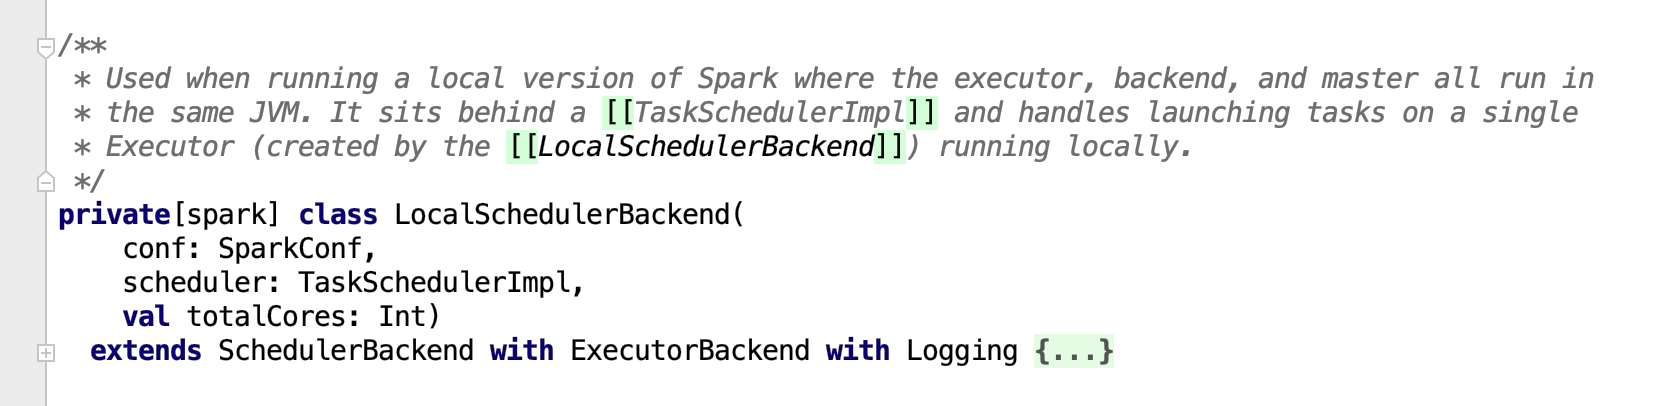
\includegraphics[width=1\linewidth]{images/init008}
		\caption{LocalSchedulerBackend}
		\label{fig:init008}
	\end{figure}
	
	
\end{frame}
\begin{frame}[plain,t]{SparkContext} %也可以使用\frametitle{节的名字}效果一样
	\structure{Spark on Yarn} \\  \vspace{2ex}
	\begin{figure}
		\centering
		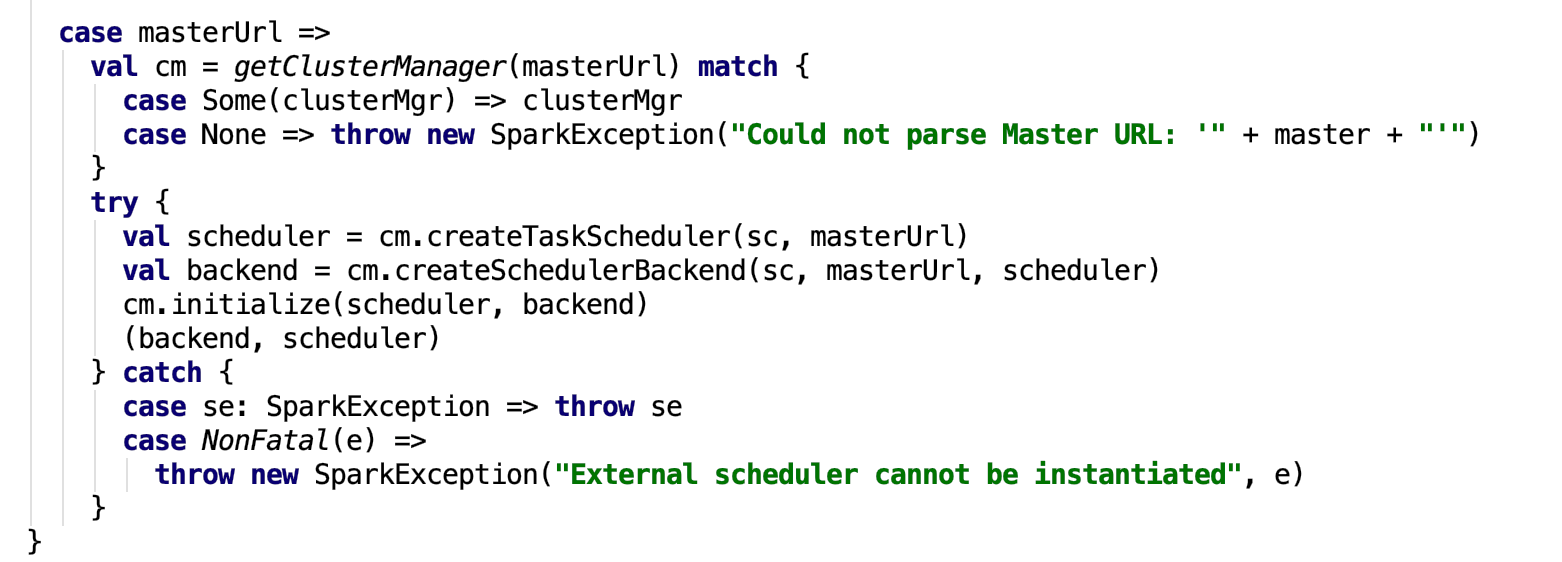
\includegraphics[width=0.9\linewidth]{images/init003}
		\caption{SparkContext\#createTaskScheduler}
		\label{fig:init003}
	\end{figure}
	
\end{frame}
\begin{frame}[plain,t]{SparkContext} %也可以使用\frametitle{节的名字}效果一样
	\structure{Spark on Yarn} \\  \vspace{2ex}
	\begin{figure}
		\centering
		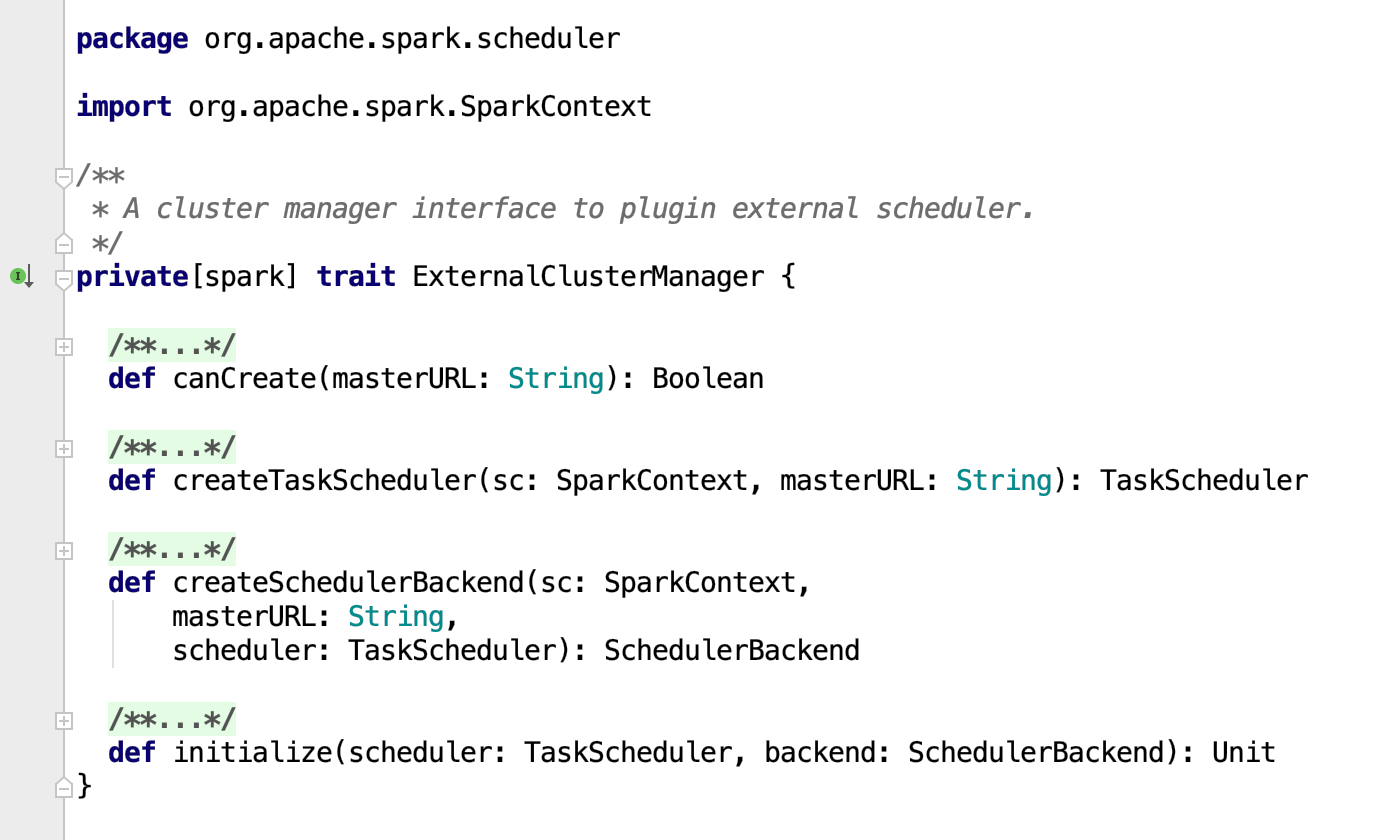
\includegraphics[width=0.9\linewidth]{images/init004}
		\caption{ExternalClusterManager}
		\label{fig:init004}
	\end{figure}
	
\end{frame}
\begin{frame}[plain,t]{SparkContext} %也可以使用\frametitle{节的名字}效果一样
	\structure{Spark on Yarn} \\ 
	\begin{figure}
		\centering
		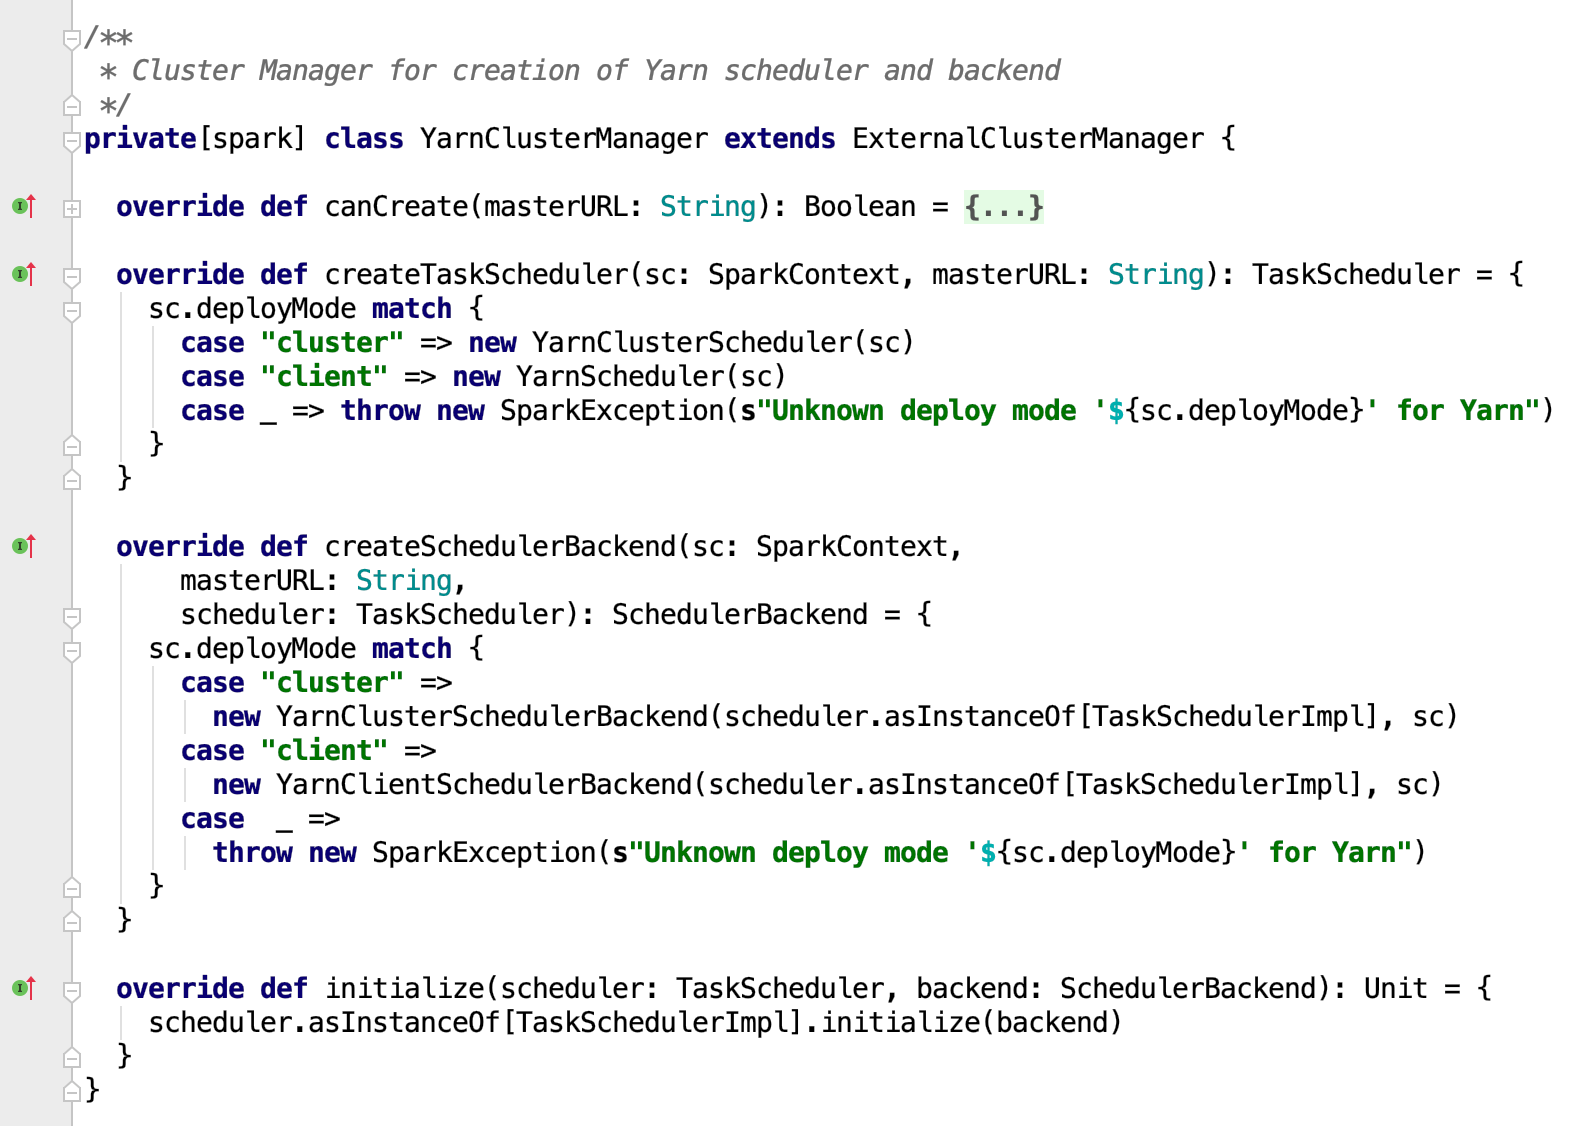
\includegraphics[width=0.9\linewidth]{images/init005}
		\caption{YarnClusterManager}
		\label{fig:init005}
	\end{figure}
	
\end{frame}
\begin{frame}[plain,t]{SparkContext} %也可以使用\frametitle{节的名字}效果一样
	\structure{Spark on Yarn} \\  \vspace{2ex}
	\begin{figure}
		\centering
		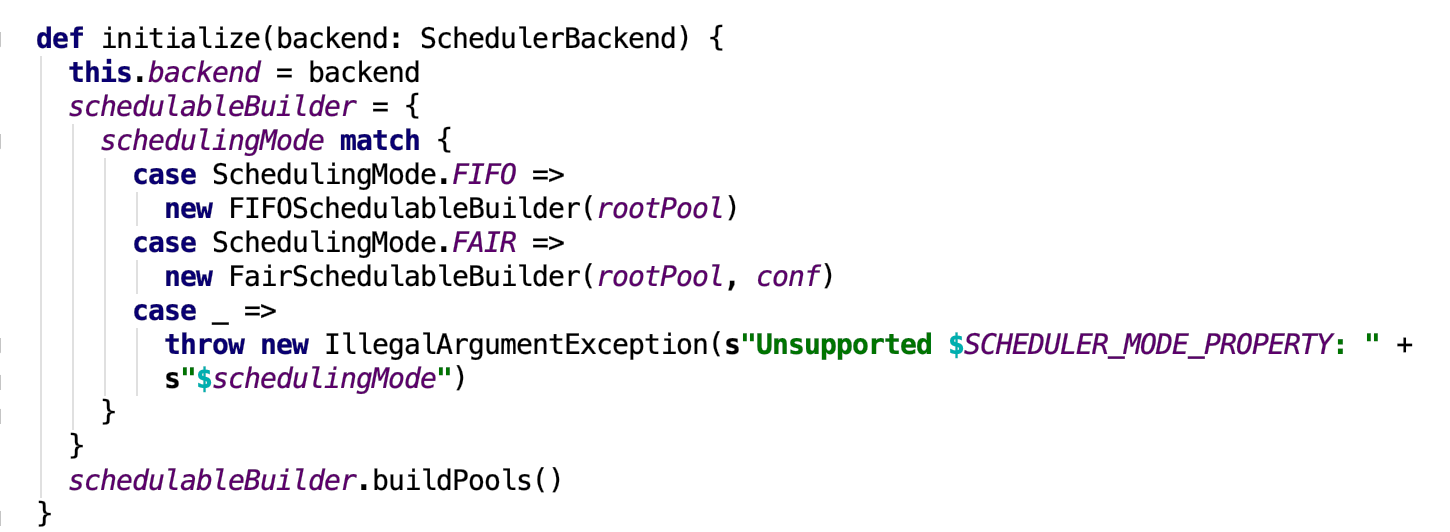
\includegraphics[width=0.9\linewidth]{images/init006}
		\caption{TaskSchedulerImpl\#initialize}
		\label{fig:init006}
	\end{figure}
	
\end{frame}
\begin{frame}[plain,t]{SparkContext} %也可以使用\frametitle{节的名字}效果一样
	\structure{Spark on Yarn} \\  \vspace{2ex}
	\begin{figure}
		\centering
		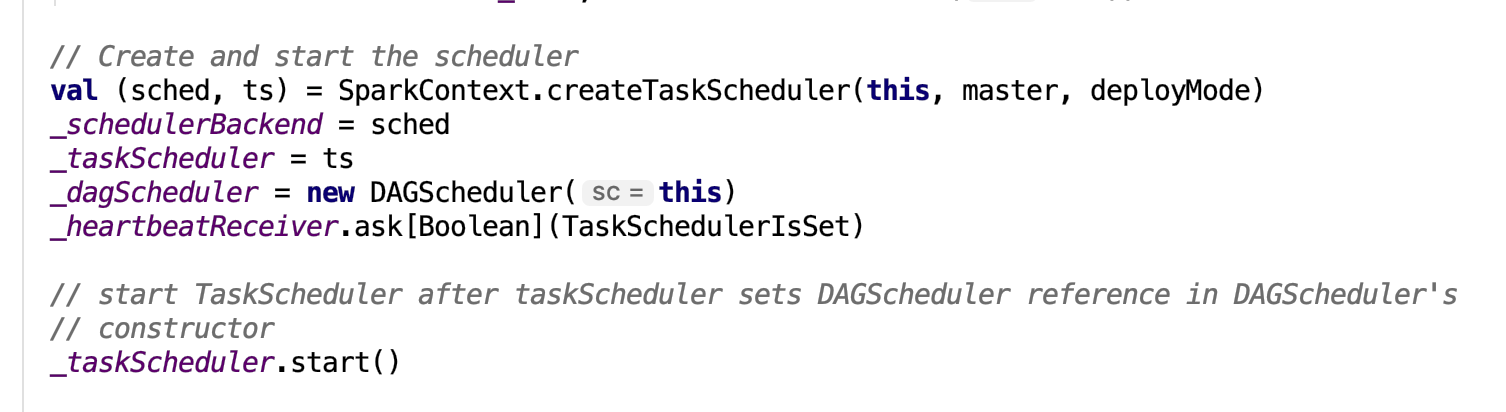
\includegraphics[width=0.9\linewidth]{images/init002}
		\caption{SparkContext\#init}
		\label{fig:init002}
	\end{figure}
	
\end{frame}
\begin{frame}[plain,t]{SparkContext} %也可以使用\frametitle{节的名字}效果一样
	\structure{Spark on Yarn} \\  \vspace{2ex}
	\begin{figure}
		\centering
		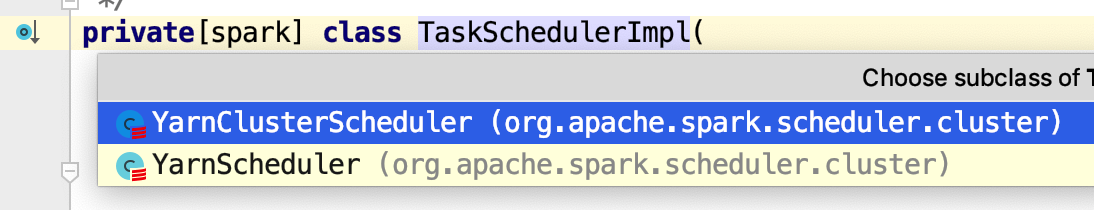
\includegraphics[width=0.9\linewidth]{images/init009}
		%\caption{TaskSchedulerImpl}
		\label{fig:init009}
	\end{figure}
\begin{figure}
	\centering
	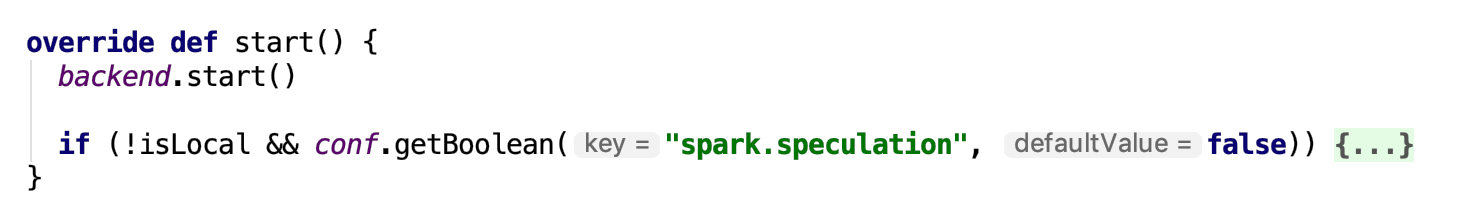
\includegraphics[width=0.9\linewidth]{images/init010}
	\caption{TaskSchedulerImpl\#start}
	\label{fig:init010}
\end{figure}

	
\end{frame}
\begin{frame}[plain,t]{SparkContext} %也可以使用\frametitle{节的名字}效果一样
	\structure{Spark on Yarn {\color{red} Cluster}} \\  
	\begin{figure}
		\centering
		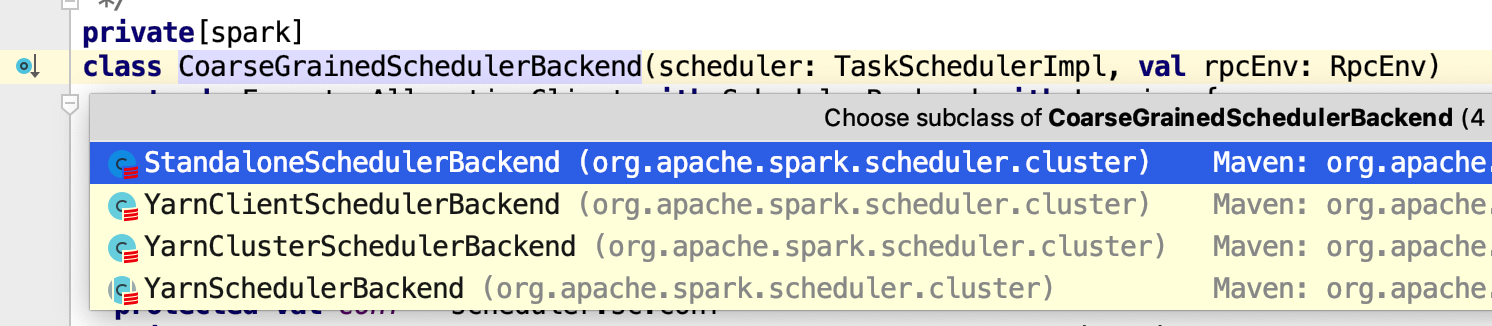
\includegraphics[width=0.9\linewidth]{images/init011}
		%\caption{}
		\label{fig:init011}
	\end{figure}

\begin{figure}
	\centering
	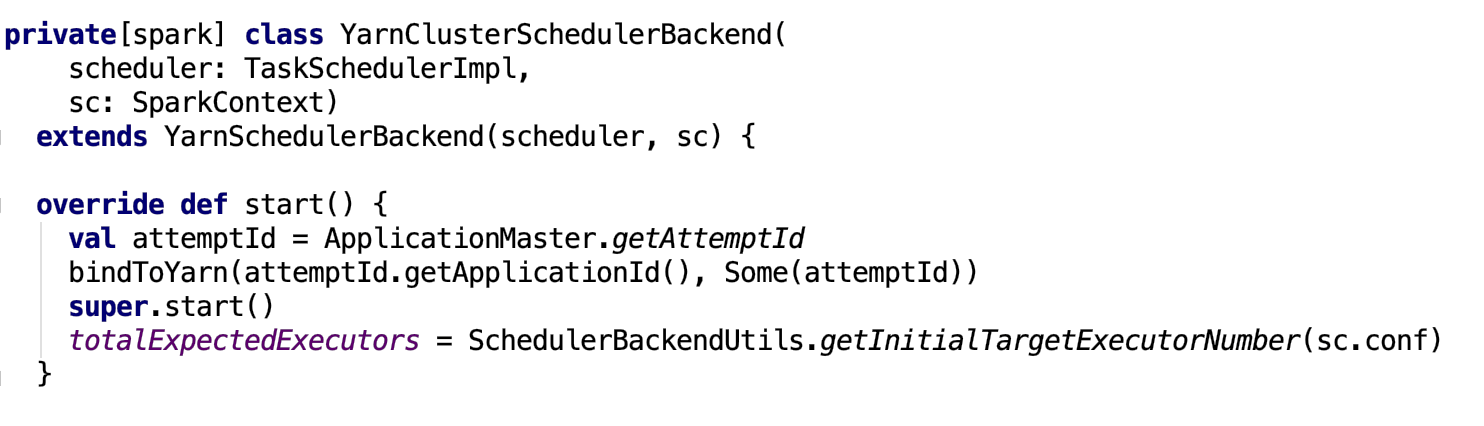
\includegraphics[width=0.9\linewidth]{images/init013}
	\caption{YarnClusterSchedulerBackend\#start}
	\label{fig:init013}
\end{figure}
\end{frame}

\begin{frame}[plain,t]{SparkContext} %也可以使用\frametitle{节的名字}效果一样
	\structure{Spark on Yarn  {\color{magenta} Client}} \\  
	\begin{figure}
		\centering
		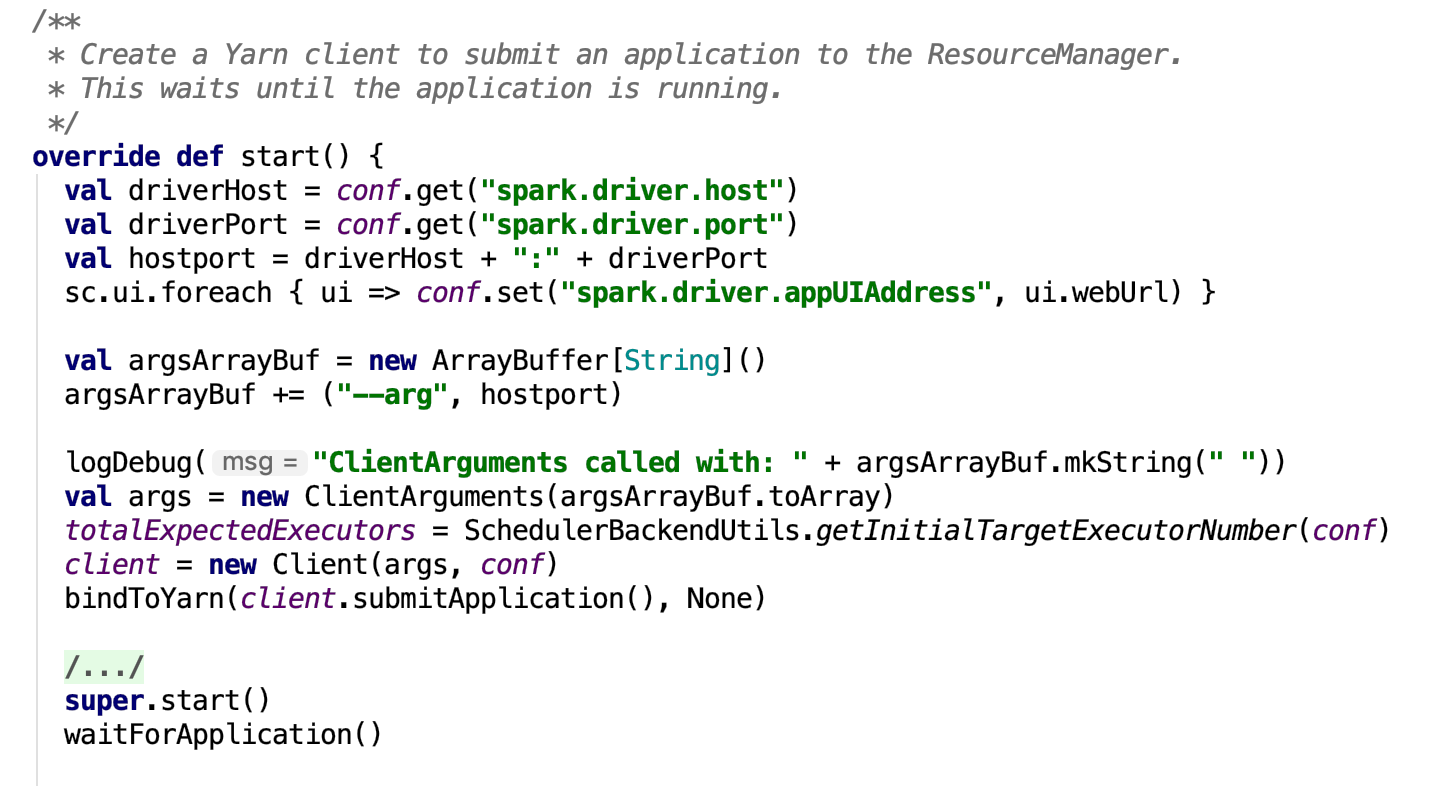
\includegraphics[width=0.9\linewidth]{images/init014}
		\caption{YarnClientSchedulerBackend\#start}
		\label{fig:init014}
	\end{figure}
\end{frame}
\begin{frame}[plain,t]{SparkContext} %也可以使用\frametitle{节的名字}效果一样
	\structure{Spark on Yarn} \\  
	\begin{figure}
		\centering
		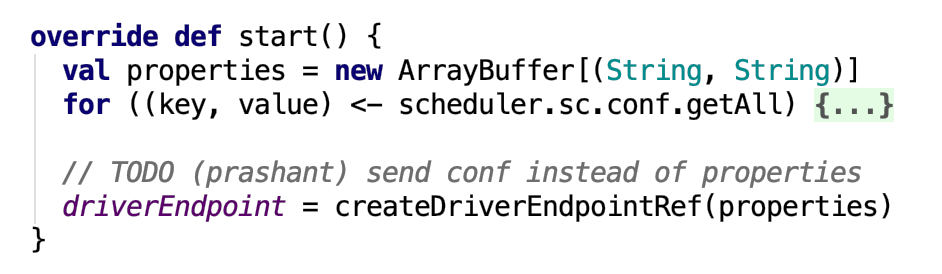
\includegraphics[width=0.9\linewidth]{images/init012}
		\caption{CoarseGrainedSchedulerBackend\#start}
		\label{fig:init012}
	\end{figure}
\end{frame}
\begin{frame}[plain,t]{SparkContext} %也可以使用\frametitle{节的名字}效果一样
	\structure{Spark on Yarn} \\  
	\begin{figure}
		\centering
		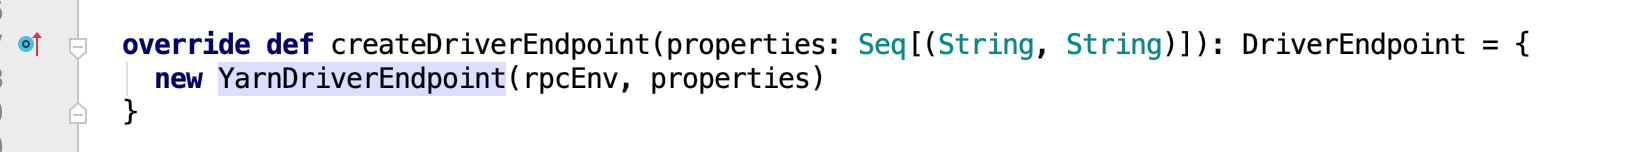
\includegraphics[width=0.9\linewidth]{images/yarn001}
		\caption{YarnSchedulerBackend\#createDriverEndpoint}
		\label{fig:yarn001}
	\end{figure}
\begin{figure}
	\centering
	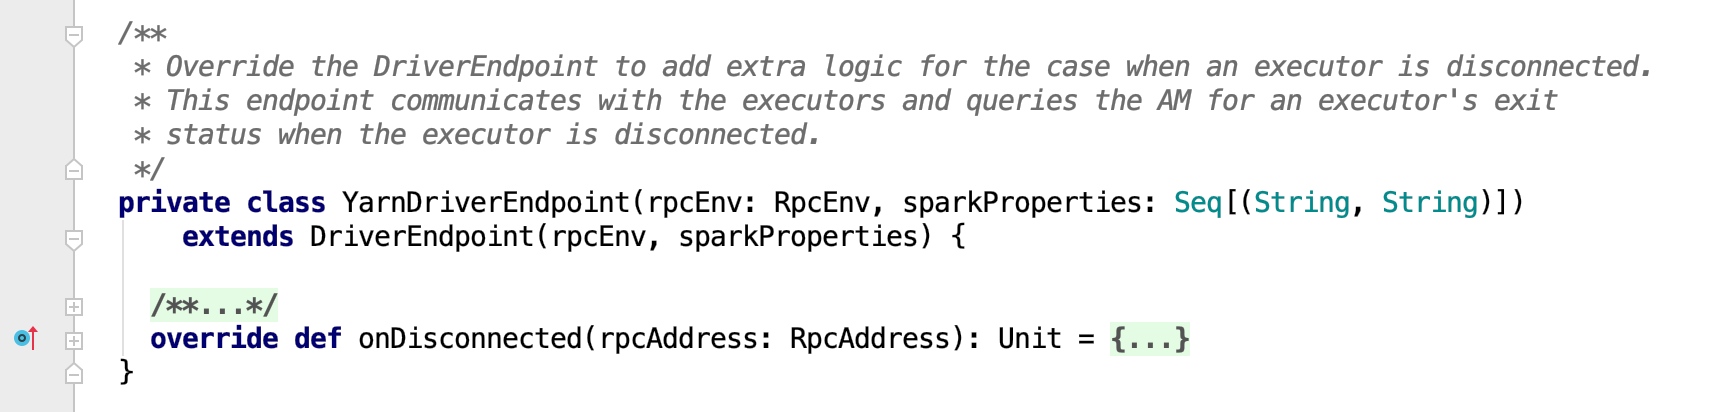
\includegraphics[width=0.9\linewidth]{images/yarn002}
	\caption{YarnDriverEndpoint}
	\label{fig:yarn002}
\end{figure}

\end{frame}
\begin{frame}[plain,t]{SparkContext} %也可以使用\frametitle{节的名字}效果一样
	\structure{Spark on Yarn} \\  
	\begin{figure}
		\centering
		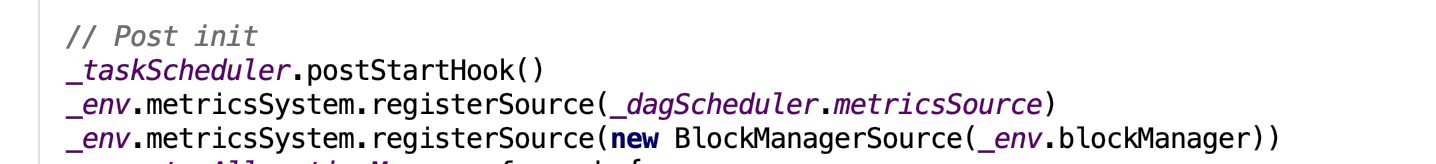
\includegraphics[width=0.9\linewidth]{images/app014}
		\caption{SparkContext\#init}
		\label{fig:app014}
	\end{figure}
	\begin{figure}
		\centering
		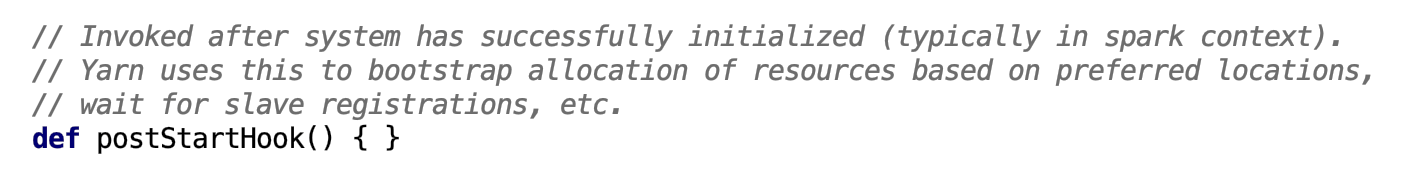
\includegraphics[width=0.9\linewidth]{images/app015}
		\caption{TaskScheduler\#postStartHook}
		\label{fig:app015}
	\end{figure}
	
	
\end{frame}


\section{Spark Scheduler}
\subsection{The high-level scheduling layer}
\begin{frame}[plain,t]{Spark Program} %也可以使用\frametitle{节的名字}效果一样
	\structure{Word Count} \\ 
	\begin{figure}
		\centering
		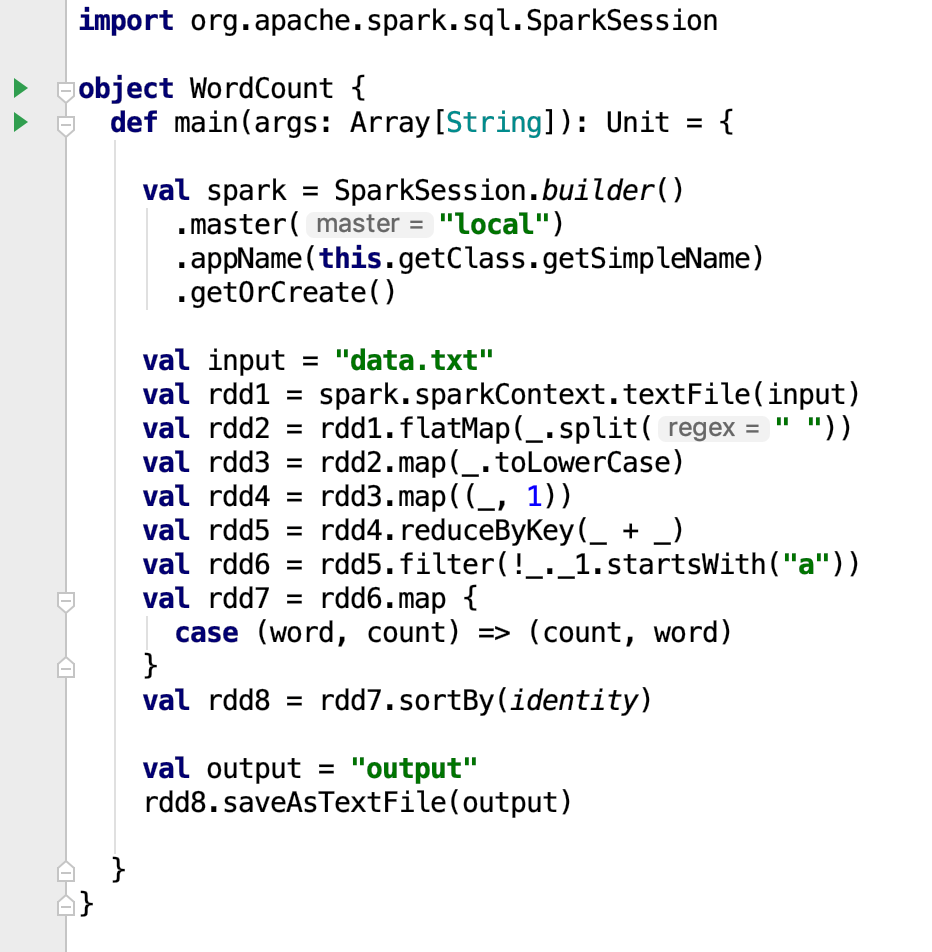
\includegraphics[width=0.65\linewidth]{images/p003}
		\caption{code}
		\label{fig:p003}
	\end{figure}
	
\end{frame}
\begin{frame}[plain,t]{Spark Program} %也可以使用\frametitle{节的名字}效果一样
	\structure{Word Count} \\  \vspace{2ex}
	\begin{figure}
		\centering
		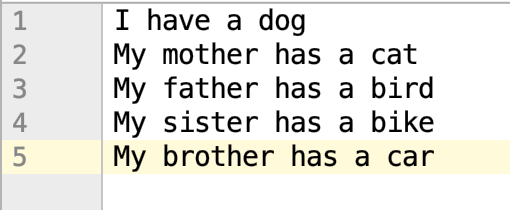
\includegraphics[width=0.9\linewidth]{images/dag013}
		\caption{data}
		\label{fig:dag013}
	\end{figure}
	
\end{frame}
\begin{frame}[plain,t]{Spark Program} %也可以使用\frametitle{节的名字}效果一样
	\structure{Word Count} \\ 
\begin{figure}
	\centering
	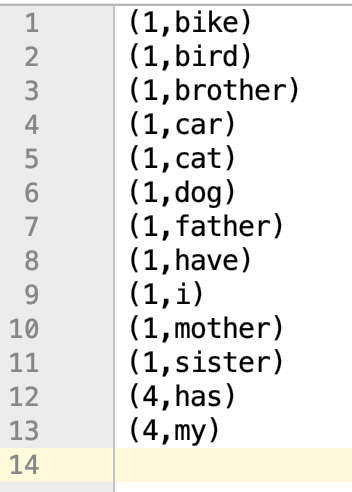
\includegraphics[width=0.45\linewidth]{images/dag014}
	\caption{result}
	\label{fig:dag014}
\end{figure}

\end{frame}



\begin{frame}[plain,t]{The  key concepts} %也可以使用\frametitle{节的名字}效果一样
	\structure{Concept} \\  \vspace{2ex}
	\begin{enumerate}
		\item Jobs
		\item Stage
		\item Task
		\item Cache tracking
		\item Preferred locations
		\item Cleanup
	\end{enumerate}
\end{frame}
\begin{frame}[plain,t]{The  key concepts} %也可以使用\frametitle{节的名字}效果一样
	\structure{Concept} \\  \vspace{2ex}
	There are three kinds of transformations:
	\begin{itemize}
		\item narrow dependencies
		\item wide dependencies
	\end{itemize}
	
	 \vspace{2ex}
	 
	There are three kinds of actions:
	\begin{itemize}
		\item Actions to view data in the console
		\item Actions to collect data to native object in the respective language
		\item Actions to write output data sources
	\end{itemize}
\end{frame}
\begin{frame}[plain,t]{The  key concepts} %也可以使用\frametitle{节的名字}效果一样
	\structure{Spark UI} \\ 
	\begin{figure}
		\centering
		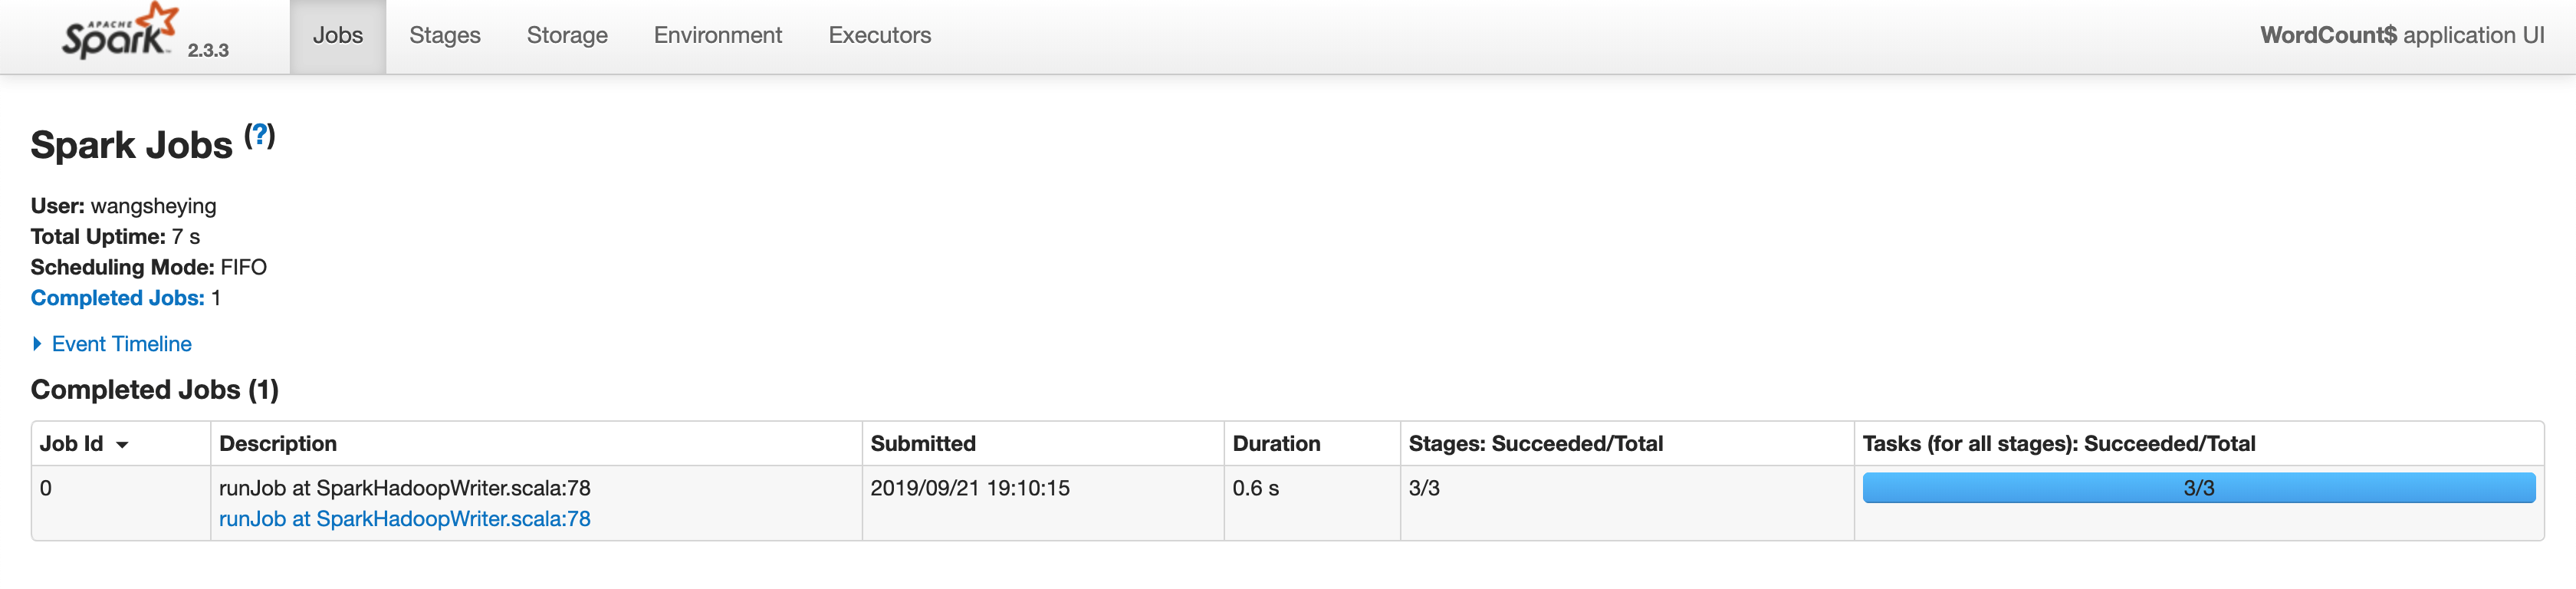
\includegraphics[width=0.9\linewidth]{images/p004}
		\caption{Job}
		\label{fig:p004}
	\end{figure}
		\begin{figure}
		\centering
		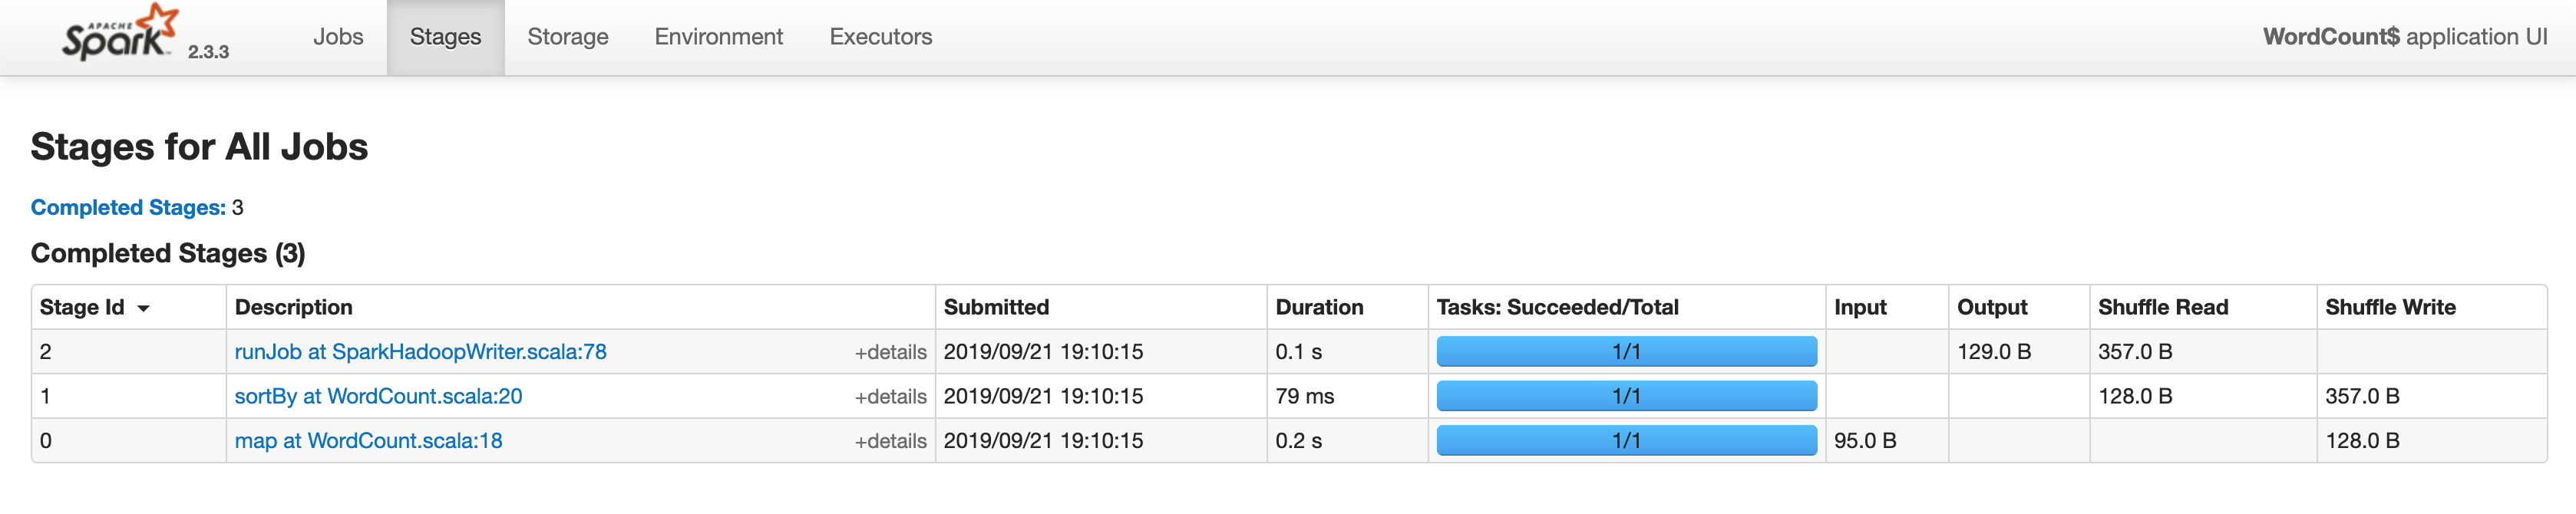
\includegraphics[width=0.9\linewidth]{images/p005}
		\caption{Stage}
		\label{fig:p005}
	\end{figure}
\end{frame}


\begin{frame}[plain,t]{The high-level scheduling layer} %也可以使用\frametitle{节的名字}效果一样
	\structure{DAGScheduler} \\  \vspace{2ex}
	The high-level scheduling layer that implements stage-oriented scheduling.
	
	\vspace{2ex}
	
	It computes a DAG of stages for each job, keeps track of which RDDs and 
	stage outputs are materialized, and finds a minimal schedule to run the job.
	
	\vspace{2ex}
	
	Spark stages are created by breaking the RDD graph at shuffle boundaries.
	
\end{frame}

\begin{frame}[plain,t]{The high-level scheduling layer} %也可以使用\frametitle{节的名字}效果一样
	\structure{DAGScheduler} \\  \vspace{2ex}

  In addition to coming up with a DAG of stages, 
  the DAGScheduler also determines the preferred locations to run each task on, 
  based on the current cache status, and passes these to the low-level TaskScheduler. 
  
  \vspace{2ex}
  
  Furthermore, it handles failures due to shuffle output files being lost, in which case old stages may need to be resubmitted.
	
\end{frame}

\begin{frame}[plain,t]{The high-level scheduling layer} %也可以使用\frametitle{节的名字}效果一样
	\structure{DAGScheduler} \\  
	
	\begin{figure}
		\centering
		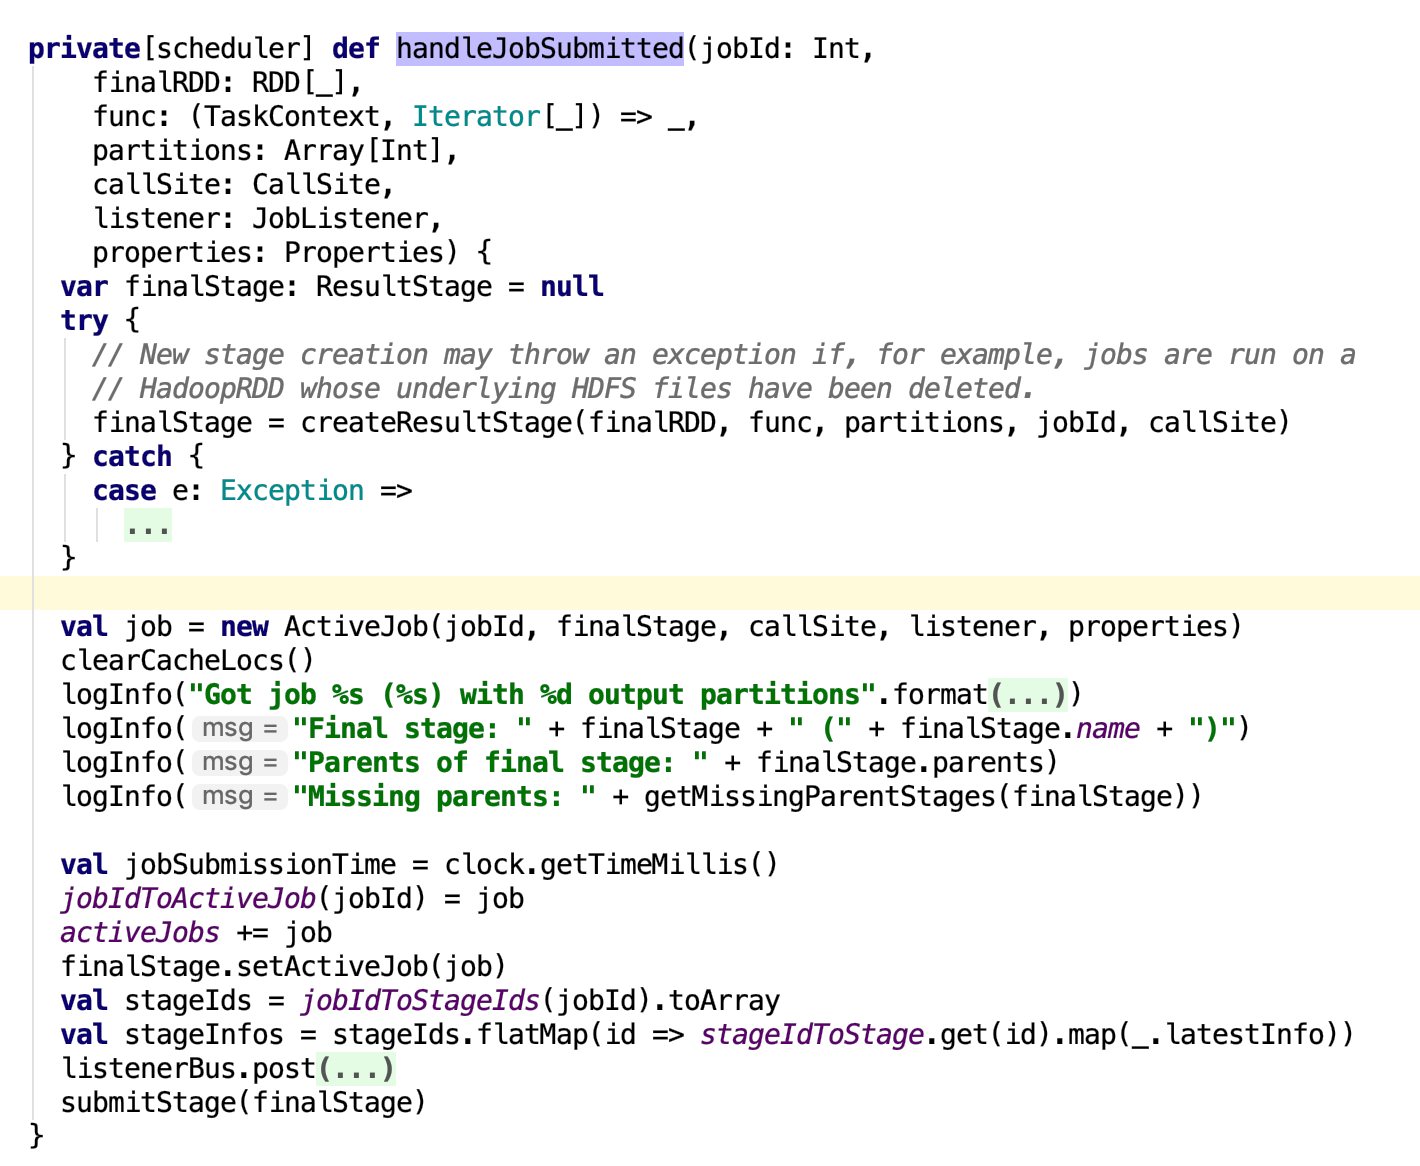
\includegraphics[width=0.8\linewidth]{images/dag002}
		\caption{DAGScheduler\#handleJobSubmitted}
		\label{fig:dag002}
	\end{figure}
\end{frame}
\begin{frame}[plain,t]{The high-level scheduling layer} %也可以使用\frametitle{节的名字}效果一样
	\structure{DAGScheduler} \\  
	\begin{figure}
		\centering
		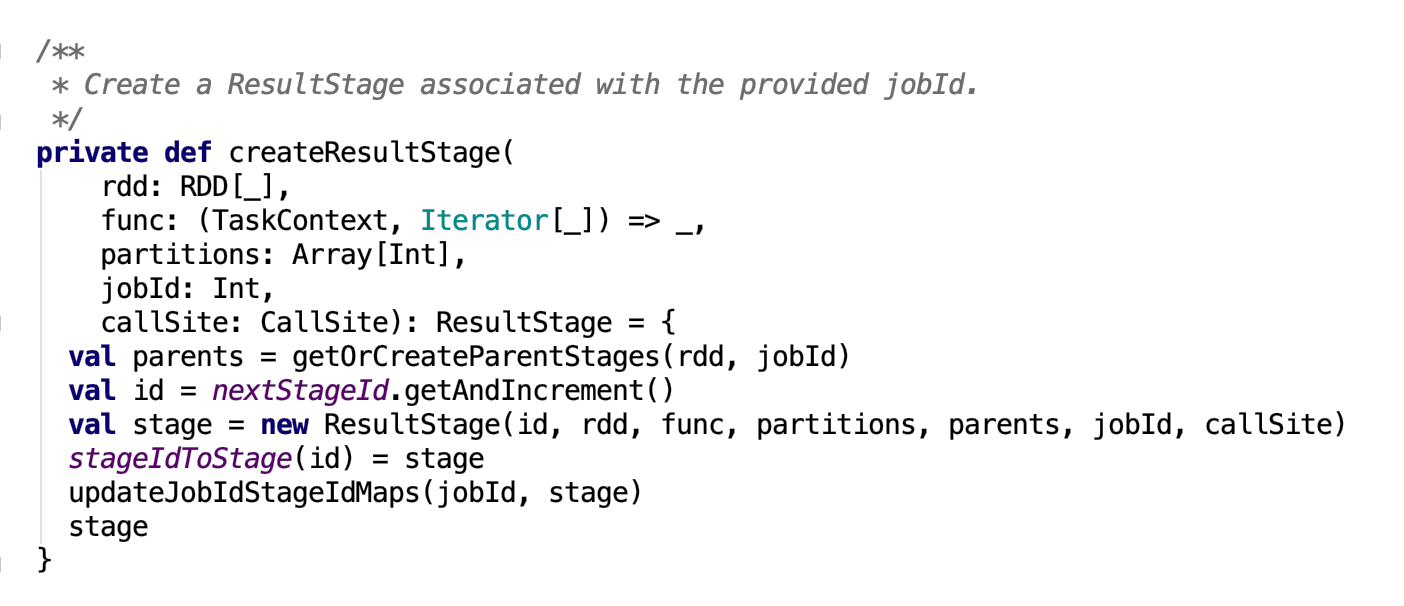
\includegraphics[width=0.9\linewidth]{images/dag007}
		\caption{DAGScheduler\#createResultStage}
		\label{fig:dag007}
	\end{figure}
	
	

\end{frame}
\begin{frame}[plain,t]{The high-level scheduling layer} %也可以使用\frametitle{节的名字}效果一样
	\structure{DAGScheduler} \\  
	\begin{figure}
		\centering
		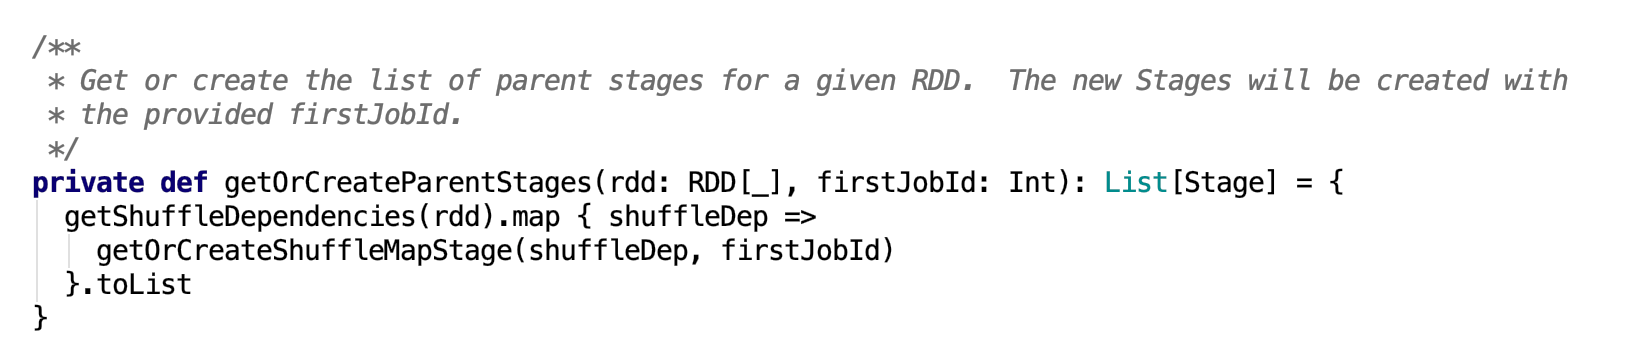
\includegraphics[width=0.9\linewidth]{images/dag008}
		\caption{DAGScheduler\#getOrCreateParentStages}
		\label{fig:dag008}
	\end{figure}
	
	
\end{frame}
\begin{frame}[plain,t]{The high-level scheduling layer} %也可以使用\frametitle{节的名字}效果一样
	\structure{DAGScheduler} \\  
	\begin{figure}
		\centering
		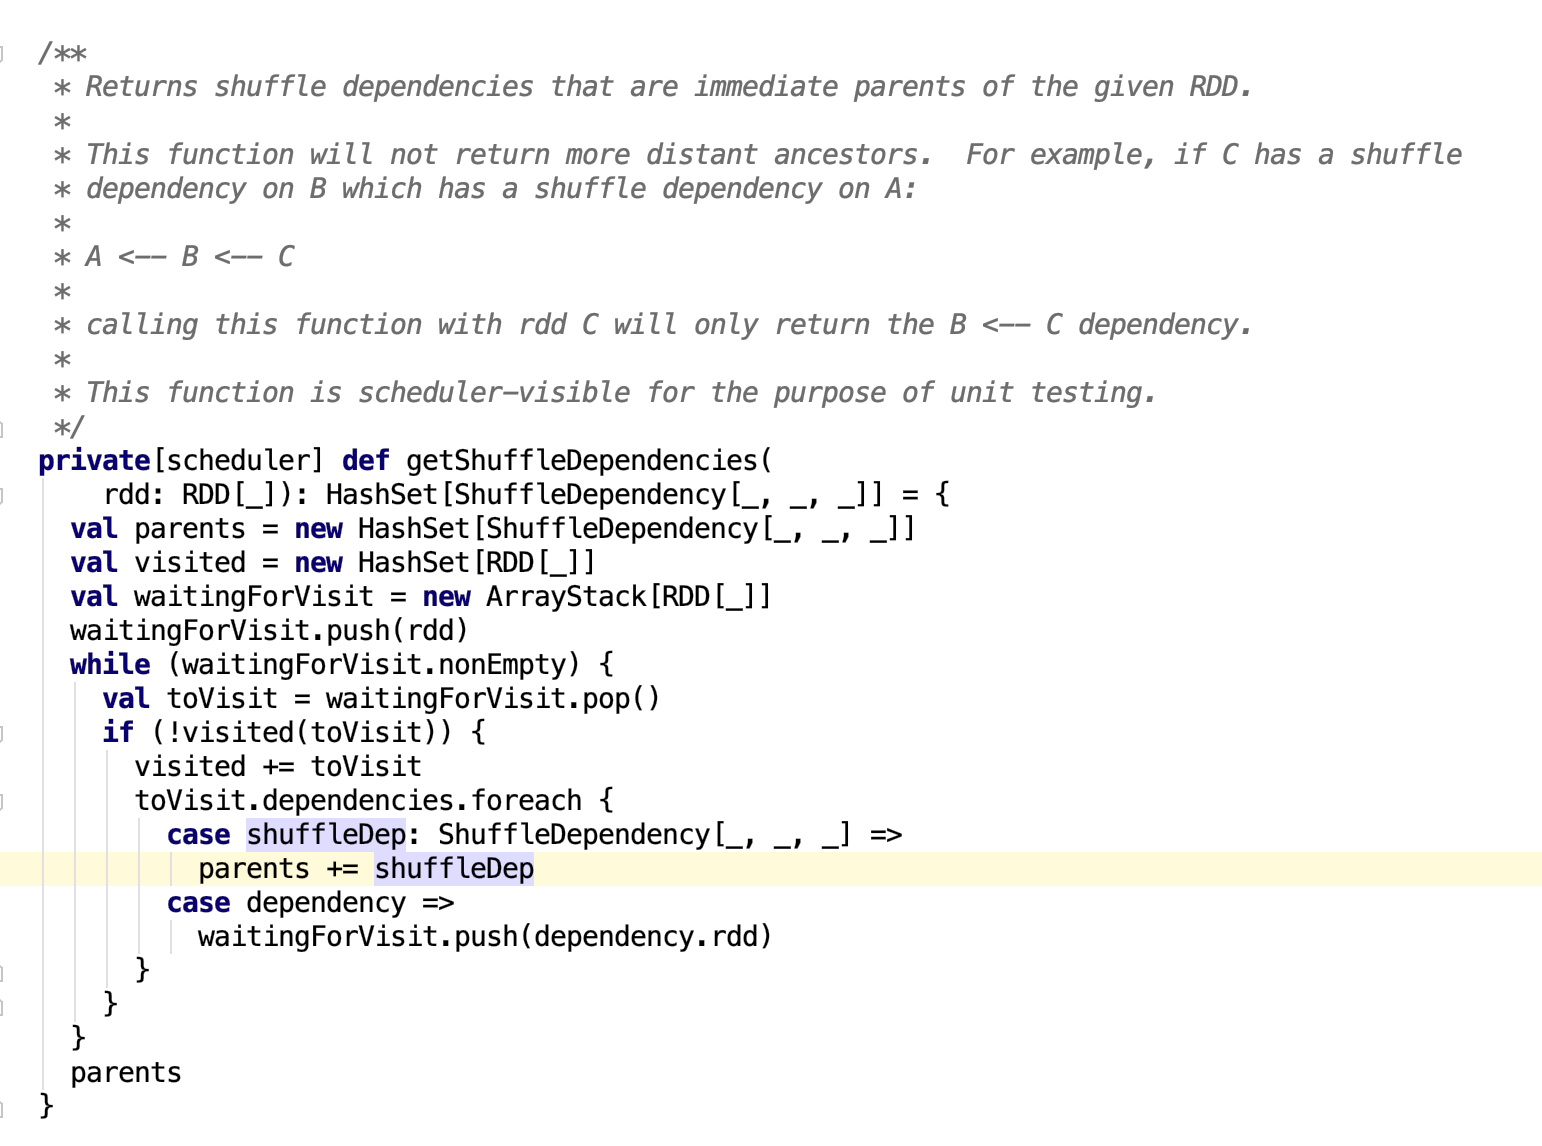
\includegraphics[width=0.9\linewidth]{images/dag009}
		\caption{DAGScheduler\#getShuffleDependencies}
		\label{fig:dag009}
	\end{figure}
	
	
\end{frame}
\begin{frame}[plain,t]{The high-level scheduling layer} %也可以使用\frametitle{节的名字}效果一样
	\structure{DAGScheduler} \\  
	\begin{figure}
		\centering
		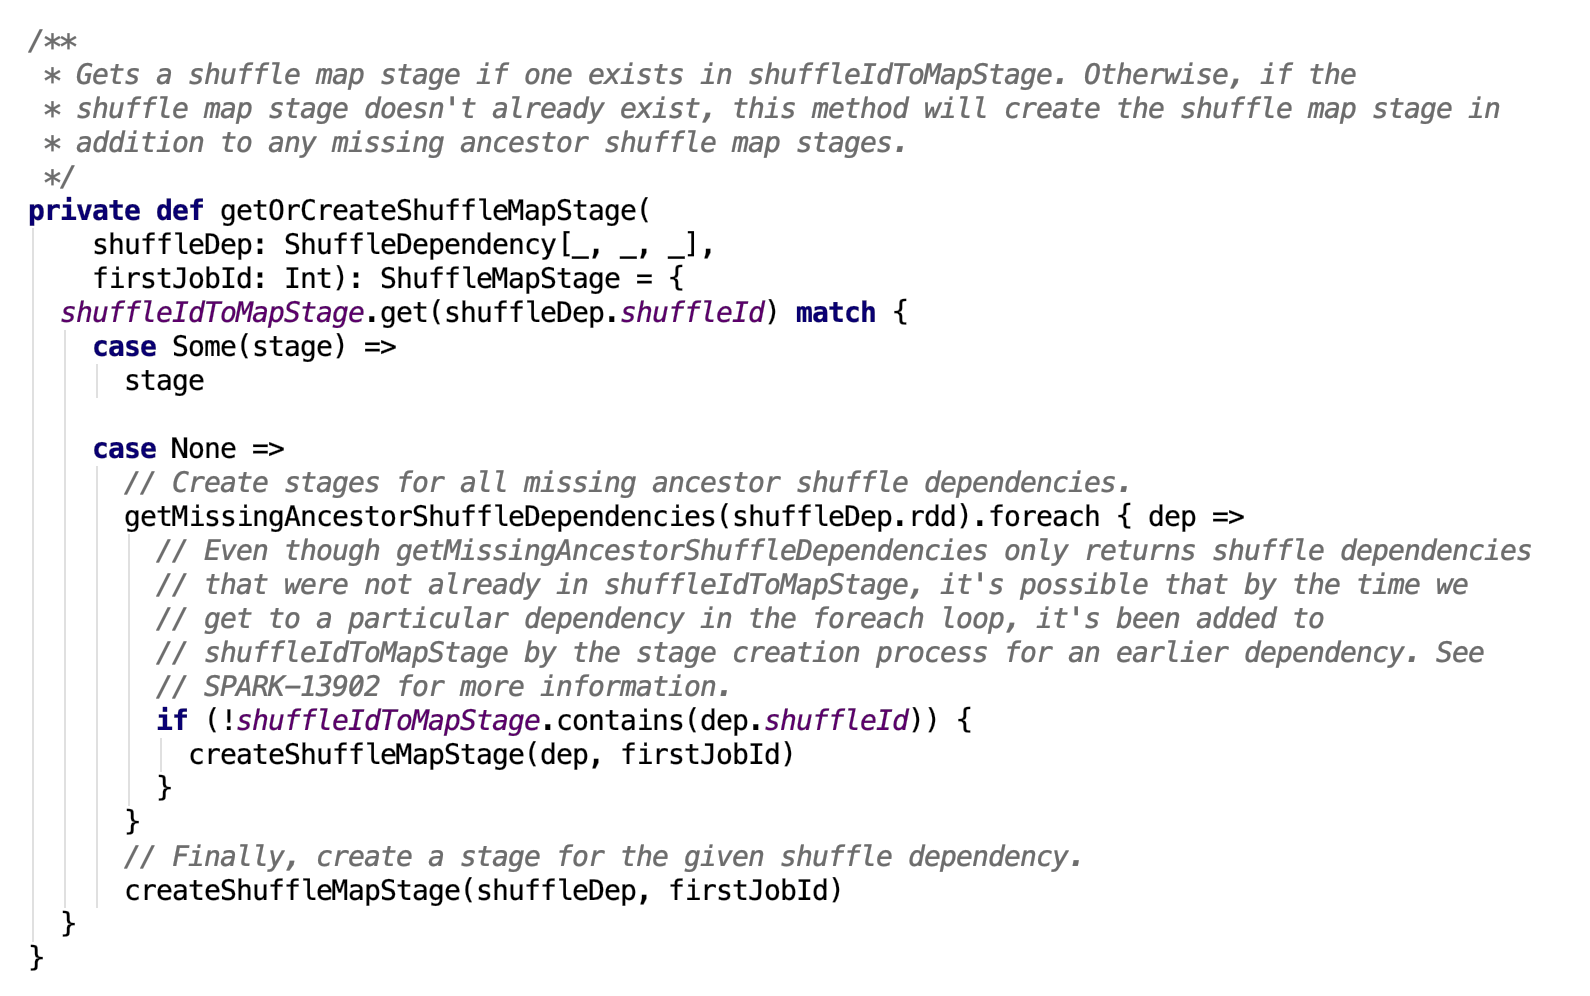
\includegraphics[width=0.9\linewidth]{images/dag010}
		\caption{DAGScheduler\#getOrCreateShuffleMapStage}
		\label{fig:dag010}
	\end{figure}
	
	
\end{frame}
\begin{frame}[plain,t]{The high-level scheduling layer} %也可以使用\frametitle{节的名字}效果一样
	\structure{DAGScheduler} \\  
	\begin{figure}
		\centering
		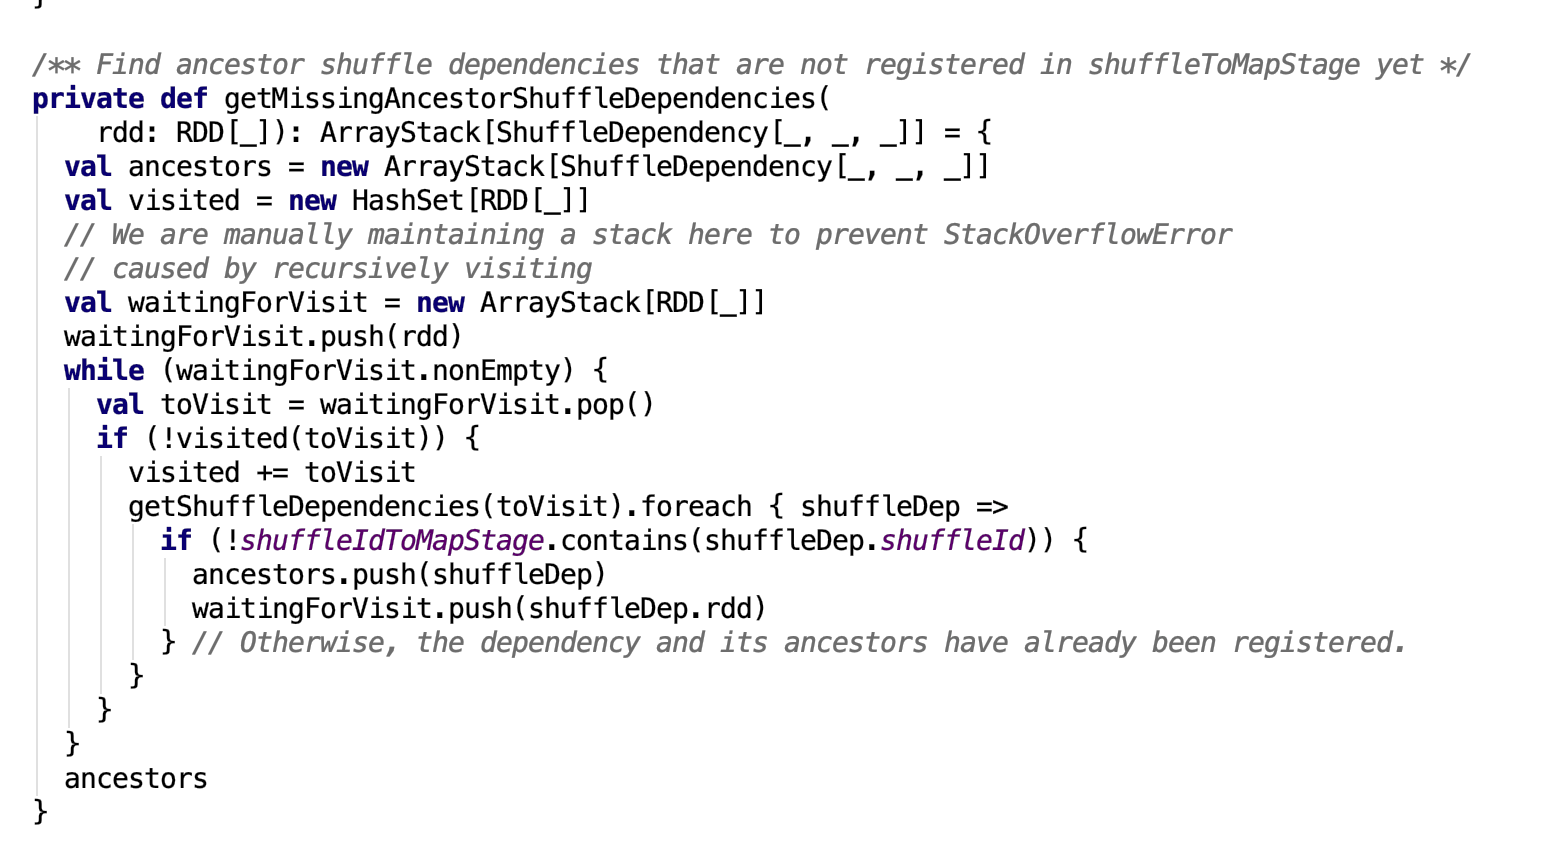
\includegraphics[width=0.9\linewidth]{images/dag011}
		\caption{DAGScheduler\#getMissingAncestorShuffleDependencies}
		\label{fig:dag011}
	\end{figure}
	
	
\end{frame}


\begin{frame}[plain,t]{The high-level scheduling layer} %也可以使用\frametitle{节的名字}效果一样
	\structure{DAGScheduler} \\  
	\begin{figure}
		\centering
		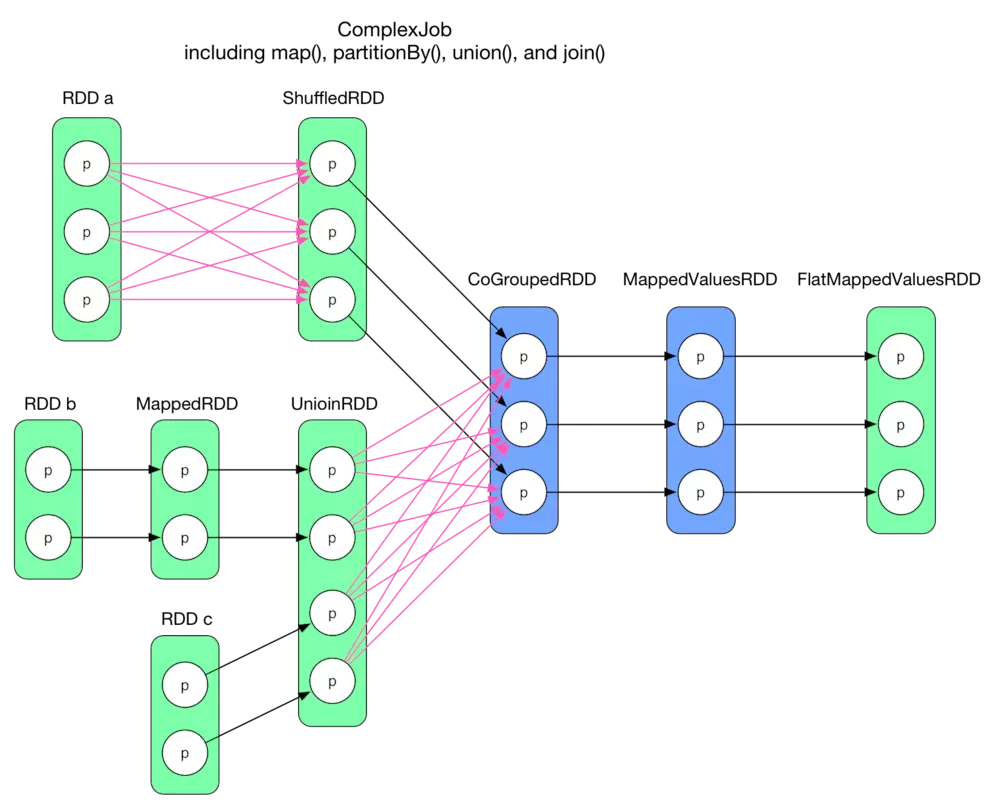
\includegraphics[width=0.9\linewidth, height=0.9\textheight]{images/dag003}
	
		\label{fig:dag003}
	\end{figure}
\end{frame}


\begin{frame}[plain,t]{The high-level scheduling layer} %也可以使用\frametitle{节的名字}效果一样
	\structure{DAGScheduler} \\  \vspace{2ex}
	It then submits stages as TaskSets to an underlying TaskScheduler implementation that runs them on the cluster.
	
	\vspace{2ex}
	
	A TaskSet contains fully independent tasks that can run right away based on the data that's already on the cluster
	 (e.g. map output files from previous stages), though it may fail if this data becomes unavailable.
	
\end{frame}
\begin{frame}[plain,t]{The high-level scheduling layer} %也可以使用\frametitle{节的名字}效果一样
	\structure{DAGScheduler} \\  
	
	\begin{figure}
		\centering
		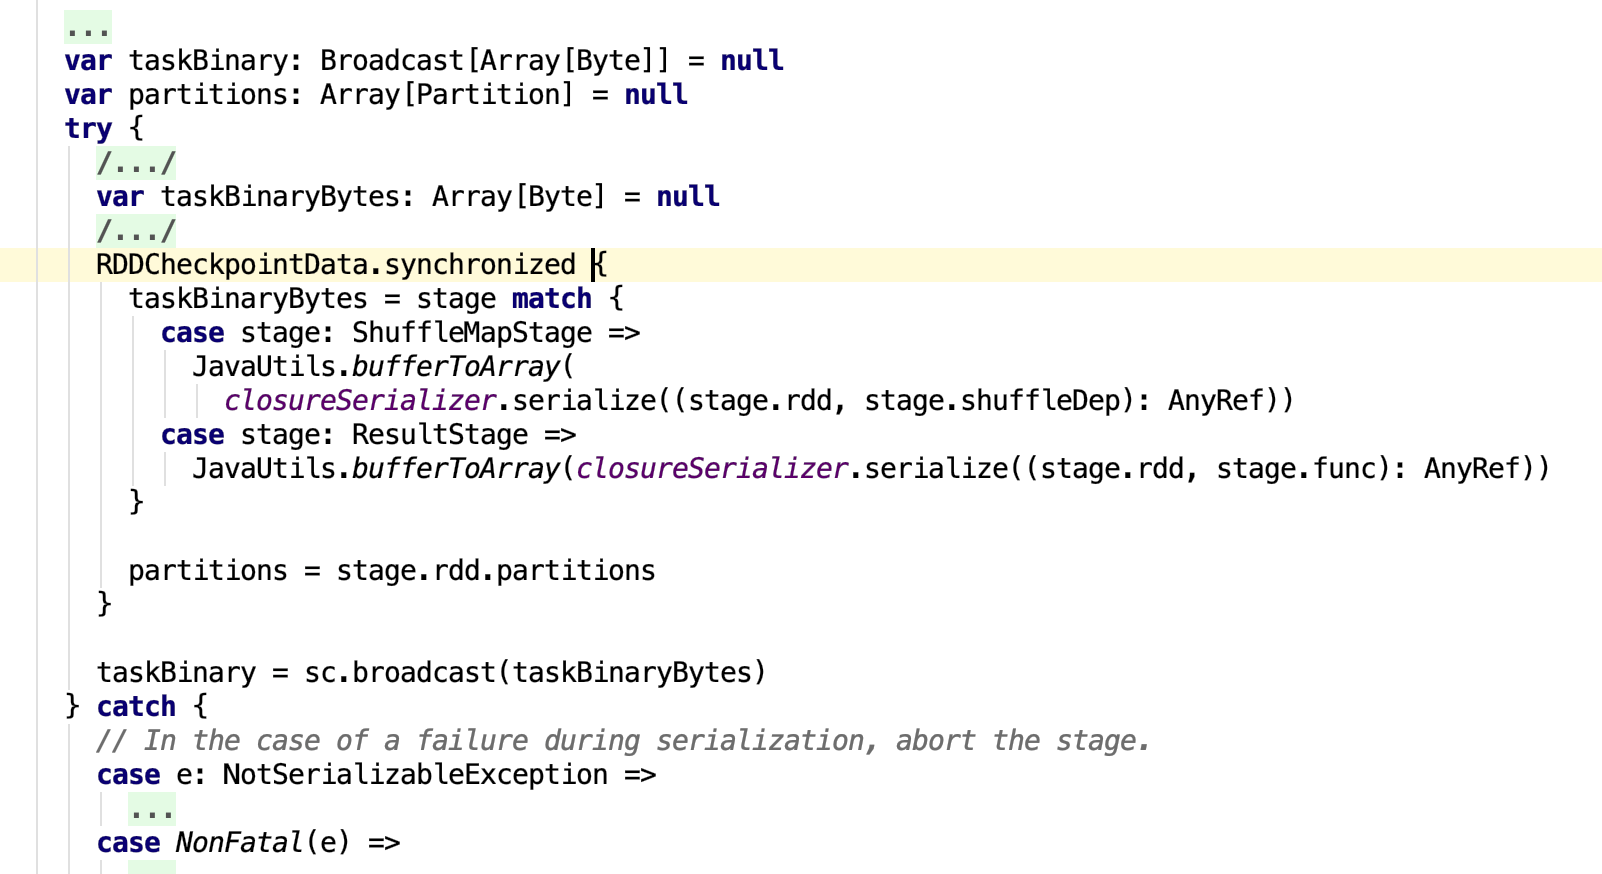
\includegraphics[width=0.9\linewidth]{images/dag004}
		\caption{DAGScheduler\#submitMissingTasks}
		\label{fig:dag004}
	\end{figure}
\end{frame}
\begin{frame}[plain,t]{The high-level scheduling layer} %也可以使用\frametitle{节的名字}效果一样
	\structure{DAGScheduler} \\  
	
	\begin{figure}
		\centering
		\includegraphics[width=0.9\linewidth]{images/dag012}
		\caption{DAGScheduler\#submitMissingTasks}
		\label{fig:dag012}
	\end{figure}
	
\end{frame}

\begin{frame}[plain,t]{The high-level scheduling layer} %也可以使用\frametitle{节的名字}效果一样
	\structure{DAGScheduler} \\  \vspace{2ex}
	\begin{figure}
		\centering
		\includegraphics[width=1\linewidth]{images/dag005}
		\caption{DAGScheduler\#submitMissingTasks}
		\label{fig:dag005}
	\end{figure}
\end{frame}

\begin{frame}[plain,t]{The Low-level scheduling layer} %也可以使用\frametitle{节的名字}效果一样
	\structure{TaskScheduler} \\  \vspace{2ex}
	\begin{figure}
		\centering
		\includegraphics[width=0.9\linewidth]{images/taskset001}
		\caption{TaskSet}
		\label{fig:taskset001}
	\end{figure}
	
\end{frame}

\begin{frame}[plain,t]{The Low-level scheduling layer} %也可以使用\frametitle{节的名字}效果一样
	\structure{TaskScheduler} \\  \vspace{2ex}
	\begin{figure}
		\centering
		\includegraphics[width=0.9\linewidth]{images/dag006}
		\caption{TaskSchedulerImpl\#submitTasks}
		\label{fig:dag006}
	\end{figure}
	
\end{frame}
\begin{frame}[plain,t]{The Low-level scheduling layer} %也可以使用\frametitle{节的名字}效果一样
	\structure{CoarseGrainedSchedulerBackend} \\  \vspace{2ex}
	
	A scheduler backend that waits for coarse-grained executors to connect.
	
	\vspace{2ex}
	
	 This backend holds onto each executor for the duration of the Spark job rather than relinquishing executors whenever a task is done and asking the scheduler to launch a new executor for  each new task.
	 
	 \begin{figure}
	 	\centering
	 	\includegraphics[width=0.9\linewidth]{images/backend001}
	 	\caption{CoarseGrainedSchedulerBackend\#reviveOffers}
	 	\label{fig:backend001}
	 \end{figure}
	 
	
\end{frame}
\begin{frame}[plain,t]{The Low-level scheduling layer} %也可以使用\frametitle{节的名字}效果一样
	\structure{DriverEndpoint} \\  \vspace{2ex}
	\begin{figure}
		\centering
		\includegraphics[width=0.9\linewidth]{images/backend002}
		\caption{CoarseGrainedSchedulerBackend.DriverEndpoint\#receive}
		\label{fig:backend002}
	\end{figure}
	
\end{frame}
\begin{frame}[plain,t]{The Low-level scheduling layer} %也可以使用\frametitle{节的名字}效果一样
	\structure{DriverEndpoint} \\  \vspace{2ex}
	\begin{figure}
		\centering
		\includegraphics[width=0.9\linewidth]{images/backend003}
		\caption{CoarseGrainedSchedulerBackend.DriverEndpoint\#makeOffers}
		\label{fig:backend003}
	\end{figure}
	
\end{frame}





\begin{frame}[plain,t]{The Low-level scheduling layer} %也可以使用\frametitle{节的名字}效果一样
	\structure{TaskScheduler} \\  \vspace{2ex}
	\begin{figure}
		\centering
		\includegraphics[width=0.9\linewidth]{images/tasksch0001}
		\caption{TaskSchedulerImpl\#resourceOffers}
		\label{fig:tasksch0001}
	\end{figure}
	
\end{frame}
\begin{frame}[plain,t]{The Low-level scheduling layer} %也可以使用\frametitle{节的名字}效果一样
	\structure{TaskScheduler} \\  
	\begin{figure}
		\centering
		\includegraphics[width=0.4\linewidth]{images/p006}
		%\caption{}
		\label{fig:p006}
	\end{figure}
\end{frame}
\begin{frame}[plain,t]{The Low-level scheduling layer} %也可以使用\frametitle{节的名字}效果一样
	\structure{DriverEndpoint} \\  \vspace{2ex}
	\begin{figure}
		\centering
		\includegraphics[width=0.9\linewidth]{images/backend004}
		\caption{DriverEndpoint\#launchTasks}
		\label{fig:backend004}
	\end{figure}
	
	
\end{frame}


\subsection{The low-level scheduling layer}
\begin{frame}[plain,t]{Executor} %也可以使用\frametitle{节的名字}效果一样
	\structure{CoarseGrainedExecutorBackend} \\  \vspace{2ex}
	\begin{figure}
		\centering
		\includegraphics[width=0.9\linewidth]{images/executor001}
		\caption{CoarseGrainedExecutorBackend\#receive}
		\label{fig:executor001}
	\end{figure}
	
	
\end{frame}
\begin{frame}[plain,t]{Executor} %也可以使用\frametitle{节的名字}效果一样
	\structure{Executor} \\  \vspace{2ex}
	\begin{figure}
		\centering
		\includegraphics[width=0.9\linewidth]{images/executor002}
		\caption{Executor\#launchTask}
		\label{fig:executor002}
	\end{figure}

  \begin{figure}
  	\centering
  	\includegraphics[width=0.9\linewidth]{images/executor003}
  	\caption{TaskRunner}
  	\label{fig:executor003}
  \end{figure}
  
\end{frame}
\subsection{Shuffle}
\begin{frame}[plain,t]{Shuffle} %也可以使用\frametitle{节的名字}效果一样
	\structure{Task} \\  \vspace{2ex}
	A ShuffleMapTask divides the elements of an RDD into multiple buckets 
	(based on a partitioner specified in the ShuffleDependency).
	
	 \vspace{2ex} 
	 
	A ResultTask that sends back the output to the driver application.
\end{frame}
\begin{frame}[plain,t]{Shuffle} %也可以使用\frametitle{节的名字}效果一样
	\structure{ShuffleMapTask} \\  \vspace{2ex}
	\begin{figure}
		\centering
		\includegraphics[width=1\linewidth]{images/maptask001}
		\caption{ShuffleMapTask\#runTask}
		\label{fig:maptask001}
	\end{figure}
	
\end{frame}
\begin{frame}[plain,t]{Shuffle} %也可以使用\frametitle{节的名字}效果一样
	\structure{ResultTask} \\  \vspace{2ex}
	\begin{figure}
		\centering
		\includegraphics[width=1\linewidth]{images/resulttask001}
		\caption{ResultTask\#runTask}
		\label{fig:resulttask001}
	\end{figure}
	
\end{frame}
\begin{frame}[plain,t]{Shuffle} %也可以使用\frametitle{节的名字}效果一样
	\structure{RDD} \\  \vspace{2ex}
\begin{figure}
	\centering
	\includegraphics[width=1\linewidth]{images/rdd001}
	\caption{RDD\#iterator}
	\label{fig:rdd001}
\end{figure}

\end{frame}
\begin{frame}[plain,t]{Shuffle} %也可以使用\frametitle{节的名字}效果一样
	\structure{RDD} \\  \vspace{2ex}
	\begin{figure}
		\centering
		\includegraphics[width=1\linewidth]{images/rdd002}
		\caption{RDD\#compute}
		\label{fig:rdd002}
	\end{figure}
	
\end{frame}
\begin{frame}[plain,t]{Shuffle} %也可以使用\frametitle{节的名字}效果一样
	\structure{RDD} \\  \vspace{2ex}
	\begin{figure}
		\centering
		\includegraphics[width=1\linewidth]{images/rdd003}
		\caption{ShuffledRDD\#compute}
		\label{fig:rdd003}
	\end{figure}
		\begin{figure}
		\centering
		\includegraphics[width=1\linewidth]{images/rdd004}
		\caption{NewHadoopRDD\#compute}
		\label{fig:rdd004}
	\end{figure}
\end{frame}
\begin{frame}[plain,t]{Shuffle} %也可以使用\frametitle{节的名字}效果一样
	\structure{ShuffleWriter} \\  \vspace{2ex}
\begin{columns}[c]  %开始进入分栏环境,居中设置
	\column{4cm}  %第一栏(左栏)宽度为8cm
	\begin{figure}
		\centering
		\includegraphics[width=1\linewidth]{images/p006}
		%\caption{}
	\end{figure}
	\column{4cm}  %第二栏(右栏)宽度为3cm
	\begin{figure}
		\centering
		\includegraphics[width=1\linewidth]{images/p008}
		%\caption{}
		\label{fig:p008}
	\end{figure}
\end{columns}
	
\end{frame}



\begin{frame}[plain,t]{Shuffle} %也可以使用\frametitle{节的名字}效果一样
	\structure{ShuffleWriter} \\  \vspace{2ex}
	\begin{figure}
		\centering
		\includegraphics[width=0.9\linewidth]{images/shufflewriter001}
		\caption{SortShuffleWriter\#write}
		\label{fig:shufflewriter001}
	\end{figure}
	
\end{frame}

\begin{frame}[plain,t]{Shuffle} %也可以使用\frametitle{节的名字}效果一样
	\structure{ShuffleWriter} \\  \vspace{2ex}
	\begin{figure}
		\centering
		\includegraphics[width=0.8\linewidth]{images/shufflewriter002}
		\caption{ExternalSorter\#insertAll}
		\label{fig:shufflewriter002}
	\end{figure}
		
\end{frame}
\begin{frame}[plain,t]{Shuffle} %也可以使用\frametitle{节的名字}效果一样
	\structure{ShuffleWriter} \\  \vspace{2ex}
	\begin{figure}
		\centering
		\includegraphics[width=0.7\linewidth]{images/s001}
		\caption{SizeTracker\#SAMPLE\_GROWTH\_RATE}
		\label{fig:s001}
	\end{figure}
	
\end{frame}
\begin{frame}[plain,t]{Shuffle} %也可以使用\frametitle{节的名字}效果一样
	\structure{ShuffleWriter} \\  \vspace{2ex}
	\begin{figure}
		\centering
		\includegraphics[width=0.7\linewidth]{images/s002}
		\caption{SizeTracker\#SAMPLE\_GROWTH\_RATE}
		\label{fig:s002}
	\end{figure}
	
\end{frame}
\begin{frame}[plain,t]{Shuffle} %也可以使用\frametitle{节的名字}效果一样
	\structure{ShuffleWriter} \\  \vspace{2ex}
	\begin{figure}
		\centering
		\includegraphics[width=0.9\linewidth]{images/shufflewriter003}
		\caption{ExternalSorter\#writePartitionedFile}
		\label{fig:shufflewriter003}
	\end{figure}
	
	
\end{frame}
\begin{frame}[plain,t]{Shuffle} %也可以使用\frametitle{节的名字}效果一样
	\structure{ShuffleReader} \\  \vspace{2ex}
	\begin{columns}[c]  %开始进入分栏环境,居中设置
		\column{4cm}  %第一栏(左栏)宽度为8cm
		\begin{figure}
			\centering
			\includegraphics[width=1\linewidth]{images/p008}
		\end{figure}
		\column{4cm}  %第二栏(右栏)宽度为3cm
		\begin{figure}
			\centering
			\includegraphics[width=1\linewidth]{images/p009}
			%\caption{}
			\label{fig:p009}
		\end{figure}
	\end{columns}
	
\end{frame}
\begin{frame}[plain,t]{Shuffle} %也可以使用\frametitle{节的名字}效果一样
	\structure{ShuffleReader} \\  \vspace{2ex}
	\begin{figure}
		\centering
		\includegraphics[width=1\linewidth]{images/shufflereader001}
		\caption{BlockStoreShuffleReader\#read}
		\label{fig:shufflereader001}
	\end{figure}
	
\end{frame}
\begin{frame}[plain,t]{Shuffle} %也可以使用\frametitle{节的名字}效果一样
	\structure{ShuffleReader} \\  \vspace{2ex}
	\begin{figure}
		\centering
		\includegraphics[width=1\linewidth]{images/suhfflereader002}
		\caption{BlockStoreShuffleReader\#read}
		\label{fig:suhfflereader002}
	\end{figure}
	
\end{frame}
\begin{frame}[plain,t]{Shuffle} %也可以使用\frametitle{节的名字}效果一样
	\structure{ShuffleReader} \\  \vspace{2ex}
	\begin{figure}
		\centering
		\includegraphics[width=1\linewidth]{images/shufflereader004}
		\caption{Aggregator}
		\label{fig:shufflereader004}
	\end{figure}
	
	
\end{frame}



\begin{frame}[plain,t]{Shuffle} %也可以使用\frametitle{节的名字}效果一样
	\structure{ShuffleReader} \\  \vspace{2ex}
	\begin{figure}
		\centering
		\includegraphics[width=1\linewidth]{images/shufflereader003}
		\caption{BlockStoreShuffleReader\#read}
		\label{fig:shufflereader003}
	\end{figure}
	
\end{frame}
\begin{frame}[plain,t]{The Final Result} %也可以使用\frametitle{节的名字}效果一样
	\structure{Actions} \\  \vspace{2ex}

	There are three kinds of actions:
	\begin{itemize}
		\item Actions to collect data
		\item Actions to write output data sources
		\item Actions to view data in the console
	\end{itemize}
\end{frame}

\subsection{Back  to the driver}
\begin{frame}[plain,t]{The Final Result} %也可以使用\frametitle{节的名字}效果一样
	\structure{Back  to the driver} \\ 
	\begin{figure}
		\centering
		\includegraphics[width=0.9\linewidth]{images/rdd006}
		\caption{RDD\#count}
		\label{fig:rdd006}
	\end{figure}
	\begin{figure}
		\centering
		\includegraphics[width=0.9\linewidth]{images/rdd007}
		\caption{SparkContext\#runJob}
		\label{fig:rdd007}
	\end{figure}
	
\end{frame}
\begin{frame}[plain,t]{The Final Result} %也可以使用\frametitle{节的名字}效果一样
	\structure{Back  to the driver} \\ 

\begin{figure}
	\centering
	\includegraphics[width=0.9\linewidth]{images/rdd010}
	\caption{SparkContext\#runJob}
	\label{fig:rdd010}
\end{figure}
	\begin{figure}
	\centering
	\includegraphics[width=0.9\linewidth]{images/rdd008}
	\caption{JobWaiter\#taskSucceeded}
	\label{fig:rdd008}
\end{figure}
	
\end{frame}
\begin{frame}[plain,t]{The Final Result} %也可以使用\frametitle{节的名字}效果一样
	\structure{Back  to the driver} \\ 
	\begin{figure}
		\centering
		\includegraphics[width=0.85\linewidth]{images/rdd009}
		\caption{DAGScheduler\#handleTaskCompletion}
		\label{fig:rdd009}
	\end{figure}
	
\end{frame}

\subsection{Write to Storage System}
\begin{frame}[plain,t]{The Final Result} %也可以使用\frametitle{节的名字}效果一样
	\structure{Write to Storage System} \\  \vspace{2ex}
	\begin{itemize}
		\item saveAsTextFile
		\item saveAsNewAPIHadoopDataset
		\item parquet
		\item foreachPartition
	\end{itemize}
	
	
\end{frame}
\subsection{View data in the console}
\begin{frame}[plain,t]{The Final Result} %也可以使用\frametitle{节的名字}效果一样
	\structure{View data in the console} \\  
	\begin{figure}
		\centering
		\includegraphics[width=0.9\linewidth]{images/p010}
		\caption{Dataset\#show}
		\label{fig:p010}
	\end{figure}
	
\end{frame}





%%=================================================================================================
\begin{frame}[plain]
	\huge
	\vfill
	\centerline{ \structure{Questions and Answers?} }
	\vfill

\end{frame}
\begin{frame}[plain]
	\huge
	\vfill
	\centerline{ \structure{Questions and Answers?} }
	\vfill
	\Huge
	\centerline{\alert{Thank You!} }
	\vfill
\end{frame}

%**********************************************************************************************
%                  上面就是正文,自己的内容
%        下面是标准的参考文献配置
%**********************************************************************************************
\begin{frame}[plain, t, allowframebreaks]{References}
	%  allowframebreaks,这个关键字可以使得参考文献自动断页,免得手动
	%  plain格式使得一帧的最上面是白色的,没有plain,会有色彩,可以试试
	%  t 使得正文不再是默认居中,而是在top,应该加上t,比较好看。
	\bibliographystyle{alpha}         %文献的格式apalike是[1],alpha是[Lam94]
	%\beamertemplatetextbibitems        %调整文献样式
	%\scriptsize                        %文献多时调整字体大小
	%\bibliography{math}                 %自己的文献
\end{frame}  
\end{document} 
%**********************************************************************************************
%        上面是标准的参考文献配置
%   参考文献的主题选择apalike,见《LaTeX入门》作者:刘海洋P423页(6-1-13)说明
%   apalike文献格式,按照美国心理协会(APA)的格式,提供基本的作者年代引用方式
%   避免完全不直观的数学编号可能造成的问题。这是因为beamer的文献格式比较特殊造成的
%  实例如下:
%\beamertemplatetextbibitems %该指令可使参考文献采用文字而不是图标的标注
%\begin{frame}[plain, t, allowframebreaks]{References}
%	\scriptsize
%	\bibliographystyle{apalike}
%	\bibliography{ZhangXiao-Smoothed_Analysis_of_Tensor_Decompositions} %文献命名规范,不要怕长
%\end{frame}

%**********************************************************************************************
%   学习LaTeX好的资料,有《LaTeX入门》《A Guide to LaTeX 4th Edition》 新浪微盘可下载  
%   《一份不太简短的LATEX介绍 》,网址 CTAN:/tex-archive/info/lshort 可下载  ,有中英文,每年更新
%   tex.stackexchange.com,一个美国的专业TeX问答网站,这个网站更灵活,受益匪浅
%   www.ctan.org            usepackage资料参考
%   www.texample.net       不常用,但是聚集了的专业绘图的LaTeX代码,比如画一个probability tree,
%   遇到问题,先百度Google,90%问题可解决,不行再上知乎提问,刘海洋老师,LaTeX专家,
%   可在 tex.stackexchange.com  同时提问,最基础的是读读上面的两本书,学会自己看文档
%   论文《Type setting mathematics for science and technology according to ISO 31/XI》
%   介绍排版中数学字体的选择
%***********************************************************************************************
